\documentclass[11pt]{aghdpl}
% \documentclass[en,11pt]{aghdpl}  % praca w języku angielskim
\usepackage[polish]{babel}
%\usepackage[english]{babel}
\usepackage[utf8]{inputenc}

% dodatkowe pakiety
\usepackage{enumerate}
\usepackage{listings}
\lstloadlanguages{TeX}

\lstset{
  literate={ą}{{\k{a}}}1
           {ć}{{\'c}}1
           {ę}{{\k{e}}}1
           {ó}{{\'o}}1
           {ń}{{\'n}}1
           {ł}{{\l{}}}1
           {ś}{{\'s}}1
           {ź}{{\'z}}1
           {ż}{{\.z}}1
           {Ą}{{\k{A}}}1
           {Ć}{{\'C}}1
           {Ę}{{\k{E}}}1
           {Ó}{{\'O}}1
           {Ń}{{\'N}}1
           {Ł}{{\L{}}}1
           {Ś}{{\'S}}1
           {Ź}{{\'Z}}1
           {Ż}{{\.Z}}1
}

%---------------------------------------------------------------------------

\author{Tomasz Landowski}
\shortauthor{T. Landowski}

\titlePL{Analiza możliwości adaptacji środowisk uruchomieniowych dla logiki biznesowej na platformach mobilnych.}
\titleEN{Analysis of possible adaptation or business logic runtimes for mobile platforms.}

\shorttitlePL{Adaptacja środowisk uruchomieniowych dla logiki biznesowej na platformach mobilnych.} % skrócona wersja tytułu jeśli jest bardzo długi
\shorttitleEN{Analysis of possible adaptation or business logic runtimes for mobile platforms.}

\thesistype{Praca dyplomowa magisterska}
%\thesistype{Master of Science Thesis}

\supervisor{dr hab. Grzegorz J. Nalepa}
%\supervisor{Grzegorz J. Nalepa PhD, DSc}

\degreeprogramme{Informatyka}
%\degreeprogramme{Computer Science}

\date{2014}

\department{Katedra Informatyki Stosowanej}
%\department{Department of Applied Computer Science}

\faculty{Wydział Elektrotechniki, Automatyki,\protect\\[-1mm] Informatyki i Inżynierii Biomedycznej}
%\faculty{Faculty of Electrical Engineering, Automatics, Computer Science and Biomedical Engineering}

\acknowledgements{Serdecznie dziękuję...}


\setlength{\cftsecnumwidth}{10mm}

%---------------------------------------------------------------------------
\setcounter{secnumdepth}{4}

\begin{document}

\titlepages
\setcounter{tocdepth}{3}
\tableofcontents
\clearpage

\chapter{Wstęp}
\label{cha:wstep}

\dots
%---------------------------------------------------------------------------

\section{Cel pracy}
\label{sec:celePracy}

Celem poniższej pracy jest \dots

%---------------------------------------------------------------------------

\section{Struktura pracy}
\label{sec:strukturaPracy}

W rodziale~\ref{cha:analizaModelowaniaProcesowBiznesowych} \dots

\chapter{Zestawienie modelowania procesów biznesowych ze specyfiką aplikacji mobilnych}
\label{cha:bpmVSMobileApplications}

Tematem niniejszej pracy magisterskiej jest analiza możliwości adaptacji środowisk uruchomieniowych dla logiki biznesowej na platformach mobilnych. Temat jest szeroki, zarówno środowiska uruchomieniowe dla logiki biznesowej jak i platformy mobilne mogą być rozumiane w różny sposób, dlatego na początku niezbędne jest uściślenie kilku kwestii. Środowiska uruchomieniowe dla logiki biznesowej w niniejszej pracy magisterskiej rozumiane będą przez technologię Modelowania Procesów Biznesowych. W przypadku platform mobilnych największa uwaga zostanie poświęcona najbardziej popularnej, opartej na systemie operacyjnym \textit{Unix} platformie mobilnej - \textit{Android}. Aby przejść do zestawienia tych dwóch technologii niezbędne jest ich poznanie i zrozumienie, dlatego w kolejnych sekcjach niniejszego rozdziału zostaną opisane wyżej wymienione technologii.


%---------------------------------------------------------------------------
\section{Modelowania Procesów Biznesowych}
\label{sec:analizaModelowaniaProcesowBiznesowych}

Modelowanie Procesów Biznesowych jest pojęciem bardzo ogólnym, nie zawiera w sobie żadnych szczegółów technicznych, określa jedynie pewne specyficzne podejście do rozwiązywania problemów informatycznych. W podejściu tym podczas analizy, główny nacisk kładziony jest na wyłonienie procesów występujących w analizowanym problemie. Proces jest tutaj rozumiany jako zbiór następujących w określonej kolejności operacji, prowadzących do osiągnięcia konkretnego celu. Najczęściej modelowanie procesów biznesowych jest rozważane w kontekście działania konkretnego przedsiębiorstwa, w którym wyłonienie procesów oraz odpowiednie nimi zarządzenie ma kluczowe znaczenie dla osiągnięcia sukcesu. 

\subsection{BPM}
\label{sec:bpm}

W literaturze pojęcie modelowania oraz zarządzanie procesami biznesowymi w kontekście przedsiębiorstw występuje pod skrótem BPM, którego angielskie rozwinięcie to Buisness Process Management (pl.  Zarządzanie Procesami Biznesowymi). Idea BPM jest bardzo popularna i szeroko rozwijana w środowisku IT, powstała nawet organizacja pod nazwą \textit{European Association of Buisness Process Managment} zajmująca się rozwojem i promocją BPM.  Na stronie internetowej organizacji znaleźć możemy oficjalną definicje BPM, która mówi, że w skład Zarządzania Procesami Biznesowymi wychodzi:
\begin{itemize}
\item projektowanie,
\item wykonywanie,
\item dokumentacja,
\item pomiar,
\item monitorowanie,
\item kontrola
\end{itemize}
zautomatyzowanych oraz niezautomatyzowanych procesów biznesowych~\cite{EAOBPMWeb}.

W środowisku IT zdarza się, że BPM traktowany jest jako osobna klasa systemów informatycznych, obok ERP, MES, CRM itd. Z punktu widzenia przedstawionej wyżej definicji trudno zgodzić się z takim podejściem, można jednak zauważyć że BPM de facto może zostać wykorzystany do realizacji każdego z wymienionych rodzajów oprogramowania lub posłużyć jako narzędzie integrujące wyżej wymienione klasy systemów, w celu stworzenia globalnego systemu zarządzania przedsiębiorstwem~\cite{wiBPMA}.

\subsection{Projektowanie procesów biznesowych}
\label{sec:projektowanieBPM}

Zdecydowanie jednym z najistotniejszych etapów w tworzeniu systemu opartego o procesy biznesowe jest etap projektowania. Jednym z najbardziej popularnych narzędzi do tego celu jest BPMN (\textit{Buisness Process Model and Notation}), które doczekało się już dwóch wersji. W kontekście niniejszej pracy magisterskiej notacja BPMN nie jest szczególnie ważna jednak została wspomniana ze względu na jej wykorzystanie w przykładach. Warto zwrócić uwagę  na fakt, że BPMN nie jest w żadnym stopniu implementacją, jest to jedynie sposób wizualizacji procesu za pomocą diagramu w postaci obrazka.

\subsection{Wykonywanie procesów biznesowych}
\label{sec:wykonywanieBPM}

Jak zostało wspomniane na samym początku Modelowanie Procesów Biznesowych jest pojęciem ogólnym nie wskazującym konkretnej technologii, która ma posłużyć do wykonania procesów biznesowych. Z definicji można jednak wnioskować, że środowiskiem do wykonywania procesów biznesowych w przedsiębiorstwach na pewno nie powinna być prosta aplikacja desktopowa czy mobilna. Biorąc pod uwagę wachlarz zastosowań BPM nie trudno dojść do wniosku, że najbardziej odpowiednim środowiskiem dla procesów biznesowych są środowiska aplikacji rozproszonych. 
Powyższe stwierdzenie potwierdza przegląd istniejących systemów uruchomieniowych dla procesów biznesowych. W ogromnej większości są to aplikacje webowe. 

\subsection{Podsumowanie}
\label{sec:podsumowanieBPM}

Z punktu widzenia niniejszej pracy magisterskiej, głównym wnioskiem płynącym z powyższego opisu BPM jest skala problemów rozwiązywanych przez to podejście oraz ich usytuowanie w środowisku aplikacji rozproszonych. 

%---------------------------------------------------------------------------
\section{Analiza aplikacji na platformy mobilne}
\label{sec:analizaAplikacjiMobilnych}

Wzrost popularności urządzeń przenośnych takich jak smatrphon czy tablet, wpłynął na powstanie specyficznej klasy systemów informatycznych, zwanych aplikacjami mobilnymi. Aplikacje mobilne cechuje ukierunkowanie na rozwiązywanie wąskiego rodzaju problemów przy pomocy urządzenia dostępnego dla użytkownika niemal 24h na dobę. Szczególną popularność zyskały aplikacje mobilne ukierunkowane na rynek globalny tzn. dla użytkownika masowego. Coraz większą popularność zyskują również aplikacje biznesowe ukierunkowane np. na wymianę danych pomiędzy pracownikami przedsiębiorstwa w celu rozwiązania konkretnego zadania. 

\subsection{Rodzaje aplikacji mobilnych}
\label{sec:rodzajeAplikacjiMobilnych}

Ze względu na rodzaj zastosowania aplikacje mobilne można sklasyfikować w następujący sposób:

\begin{itemize}
\item Samodzielne aplikacje -- aplikacje wykorzystujące tylko i wyłącznie lokalne zasoby urządzenia, korzystające z lokalnej bazy danych bez połączenia z systemami zewnętrznym, często nie wymagające połączenie do internetu. Dobrym przykładem takiej aplikacji może być prosty notatnik.  
\item Aplikacje klienckie -- są to aplikacje bazujące na komunikacji z systemami zewnętrznymi przy pomocy jakiegokolwiek interfejsu komunikacyjnego,  najczęściej połączenia HTTP. Zazwyczaj aplikacje te wykorzystują również lokalną bazę danych umożliwiając użytkownikom pracę z aplikacją w przypadku braku połączenia z systemem zewnętrznym.
\item Internetowe -- najczęściej strony www, aplikacje  te nie wykorzystują lokalnych zasobów urządzeń mobilnych, ich rolą jest udostępnienie prostego interfejsu użytkownika systemu dla użytkowników aplikacji mobilnych.
\item Gry  -- szczególny przypadek samodzielnych aplikacji ukierunkowanych głównie na wykorzystanie lokalnych zasobów urządzenie w celach rozrywkowych, szczególnie eksploatowana w tego typu aplikacjach jest karta graficzna urządzenia.
\end{itemize}

\subsection{Tryby online/offline}
\label{sec:trybyAplikacjiMobilnych}

Najbardziej docenianym rodzajem aplikacji mobilnych z punktu widzenia biznesu są aplikacje klienckie. W przypadku tych aplikacji bardzo istotny jest problem połączenia z systemami zewnętrznymi. Wyróżniamy tutaj dwa tryby pracy aplikacji:

\begin{itemize}
\item Tryb online -- urządzenie udostępnia przynajmniej jeden typ komunikacji bezprzewodowej (Wi-fi, Bluetooth, łącza podczerwieni (IrDa), GPRS). W trybie online aplikacje mobilne mają bezpośredni dostęp do zewnętrznych i zdalnych źródeł danych, innych urządzeń mobilnych lub stacjonarnych systemów komputerowych.   
\item Tryb offline -- urządzenie ma bezpośredni dostęp tylko do lokalnie przechowywanych informacji. Dane te mogą być jednak synchronizowane z innymi urządzeniami w czasie krótkich sesji komunikacyjnych. Wymiana danych podczas synchronizacji może następować w obu kierunkach. 
\end{itemize}

\subsection{Cechy specyficzne dla aplikacji mobilnych }
\label{sec:cechyAplikacjiMobilnych}

Opisując aplikacje mobilnie nie można zapomnieć o cechach specyficznych, które są niezwykle ważne z punktu widzenia projektanta i programisty aplikacji mobilnych. To właśnie dzięki tym cechom aplikacje mobilne posiadają tę, a nie inną specyfikę:

\begin{itemize}
\item Ograniczone zasoby sprzętowe -- urządzenie przenośnie pod względem zasobów sprzętowych nigdy nie zastąpią komputerów stacjonarnych, a tym bardziej urządzeń serwerowych. Właśnie ze względu na tę cechę aplikacje mobilne ukierunkowane są na rozwiązywanie małych - jednostkowych problemów. Projektant aplikacji mobilnych powinien szczególnie zwrócić uwagę na ten aspekt w przypadku projektowania interfejsu do komunikacji z systemami zewnętrznymi. Asplikacje mobilne powinny wykorzystywać lekkie interfejsy komunikacyjne np. REST, aby jak najmniej obciążać kartę sieciową urządzenia. 
\item Uproszczony interfejs użytkownika dostosowany do ekranów dotykowych -- cecha ta jest bardzo ważna głównie dla projektantów graficznych, ale ma również znaczący wpływ na rodzaj zadań rozwiązywanych za pomocą aplikacji mobilnych.  
\item Przerwy w działaniu aplikacji -- aplikacje mobilne w przeciwieństwie do innych rodzajów systemów są szczególnie narażone na przerwy w działaniu. Najprostszym przykładem może być rozmowa telefoniczna przychodząca w trakcie pracy z aplikacją. Najczęściej w takich przypadkach aplikacje przechodzą w tryb uśpienia i nie ma pewności czy praca zostanie wznowiona. Programiści powinny pamiętać o zapamiętywaniu poszczególnych stanów aplikacji aby użytkownik nie tracił wykonanej pracy. 
\item Dostęp do geolokalizacji -- aplikacje mobilne oprócz ograniczeń posiadają również wiele cech dodatkowych, wyróżniających je wśród innych systemów - jedną z nich jest dostęp do  geolokalizacji.  Funkcjonalność ta bardzo szeroko wykorzystywana jest przez systemy zwane \textit{Context Aware Middleware}~\cite{ContextAwareMobility}. 
\item Dostęp do aparatu/kamery -- jest to kolejna cecha rozszerzająca możliwości aplikacji mobilnych, może być wykorzystana na przykład jako narzędzie do skanowania kodów kreskowych, albo sposób dokumentacji pracy wykonanej przez użytkownika systemów mobilnych. 
\item Specyficzna architektura dla różnych systemów operacyjnych -- przyglądając się najbardziej popularnym platformą mobilnym można odnaleźć bardzo wiele cech współnych, mimo wszystko platformy te korzystają zazwyczaj z różnych technologii do realizacji podobnych celów.
\end{itemize}

\subsection{Komunikaty Push}
\label{sec:push}

Ze względu na zmienne warunki w dostępie do mediów komunikacyjnych, aplikacji mobilne wykorzystują w głównej mierze komunikacje typu pull (pobieranie informacji na żądanie) to wymiany informacji z systemami zewnętrznymi. Najpopularniejsze platformy mobilne jak \textit{Android}, \textit{iOS} oraz \textit{Windows Phone} udostępniają również alternatywny sposób komunikacji - push. 

Komunikacja push odbywa się jednak zawsze za pośrednictwem serwisów udostępnianych przez platformy mobilne do tego celu. Komunikacja ta posiada wiele ograniczeń, a już na pewno najważniejszym z nich jest brak pewności, że komunikat zostanie dostarczony. Komunikacja push powinna być zatem wykorzystywana jedynie do notyfikacji użytkownika o jakimś zdarzeniu, a nie do przesyłania informacji kluczowych dla działania aplikacji. 


%---------------------------------------------------------------------------
\section{BPEL „inteligentne” narzędzie integracyjne}
\label{sec:bpel}

BPEL (\textit{Business Process Execution Language}), a właściwie pełna nazwa WS-BPEL,  której rozwinięcie to \textit{Web Services Business Process Execution Language} jest językiem opartym o składnię XML, służącym do wykonywania procesów biznesowych w środowisku usług sieciowych. Język BPEL jest ustandaryzowany przez oranizacje OASIS (\textit{Organization for the Advancement of Structured Information Standards}). 

Organizacja OASIS definiuje język BPEL jako: \textit{Umożliwiający użytkownikom opis aktywności procesów biznesowych jako usługi sieciowe oraz definicję w jaki sposób usługi te mogę być połączone między sobą w celu wykonania zadania}~\cite{OASISweb}.

Jak argumentuje OASIS, język BPEL powstał z konieczności stworzenia dodatkowej warstwy integracyjnej, która wykorzysta potencjał dostarczony przez usługi sieciowe oraz procesy biznesowe. Warto tutaj wspomnieć o historii powstania BPEL. Microsoft i IBM dostrzegając potrzebę stworzenia technologii pozwalającej definiować przepływ wywołań usług sieciowych stworzyli osobne, ale bardzo podobne języki nazwane WSFL (\textit{Web Service Flow Language}) oraz Xlang. W miare wzrostu popularności BPM zdecydowali się połączyć siły aby stworzyć wspólny standard, opisanych za pomocą WSDL. Zarówno Microsoft jak i IBM dostrzegli, że architektura SOA (\textit{Service Oriented Architecture}) wymaga wprowadzenia technologi, która pozwoli składać klocki jakimi są usługi sieciowe w jedną zgrabną całość.

Dotychczasowy model komunikacji udostępniany przez usługi sieciowe był niewystarczający, głównie z powodu braku zachowania stanu podczas prostej komunikacji żądanie-odpowiedź.  Komunikacja ponadto była głównie jednokierunkowa. Model komunikacji dla biznesu wymagał natomiast sekwencyjnej wymiany wiadomości pomiędzy wieloma węzłami. Operacje wykonywane na węzłach mogły trwać bardzo długo, dlatego zainstaniała konieczność obsługi tego typu sytuacji przy pomocy asynchronicznego wywoływania serwisów~\cite{OASISBPELSpec}.

\subsection{Cechy języka BPEL}
\label{sec:bpelFeatures}

\begin{itemize}
\item Definiowane procesy biznesowe komunikują się z usługami sieciowymi przy pomocy WSDL 1.1 i same są usługami sieciowymi opisanymi przez WSDL 1.1.  
\item Do komunikacji pomiędzy usługami wykorzystywany jest protokół SOAP.
\item Procesy zdefiniowane są w języku bazującym na XML.
\item BPEL dostarcza funkcji do wykonywania prostych manipulacji na danych.
\item Posiada wsparcie do identyfikowania instancji procesów.
\item Posiada wsparcie dla podstawowego cyklu życia procesu.
\item Wspiera transakcyjność przy wykorzystaniu podstawowych technik takich jak akcje kompensacyjne.
\end{itemize}

\subsection{Orkiestracja czy choreografia?}
\label{sec:bpelOrchestration}
BPEL jest językiem orkiestracji usług sieciowych, a nie choreografii. Podstawowa różnica polega na tym, że w choreografii usługi współpracują ze sobą bezpośrednio. W orkiestracji usługa komunikuje się wyłącznie z menedżerem orkiestracji (w tym przypadku: maszyna BPEL), który wie, gdzie i jak przekazać dalej komunikaty. Nie musi tym samym znać innych usług biorących udział w procesie. 

Korzyści płynące z tego, że BPEL jest warstwa orkiestracji to ~\cite{wiao}:

\begin{itemize}
\item podejście integracyjne do komunikacji pomiędzy aplikacjami, które uniezależnia aplikacje od siebie,  
\item umożliwia sterowanie przepływem, zarządzanie bezpieczeństwem oraz niezawodność komunikacji,
\item co najważniejsze sposób zarządzanie i monitorowania procesów jest scentralizowany. 
\end{itemize}

\subsection{Silniki uruchomieniowe WS-BPEL}
\label{sec:bpelEngines}

WS-BPEL dostarcza jedynie opisu w jaki sposób proces ma przebiegać oraz z jakimi usługami ma się komunikować, potrafi również zdefiniować proste operacje proceduralne jak tworzenie zmiennych, operacje przypisania, warunki czy pętle. Język sam w sobie jednak nie ma zbyt wielkiej wartości bez odpowiedniego środowiska uruchomieniowego. Procesy BPEL można traktować jako skrypty interpretowane, wykonywane przez maszyny procesów biznesowych w środowisku zgodnym ze standardem BPEL. 

Najbardziej popularne środowiska uruchomieniowe BPEL to:

\begin{itemize}
\item \textit{ActiveVOS} 
\item \textit{Apache ODE}
\item \textit{ExpressBPEL BPM}
\item \textit{BizTalk Server}
\item \textit{Open ESB}
\item \textit{Oracle BPEL Process Manager}
\item \textit{OW2 Orchestra}
\item \textit{Parasoft BPEL Maestro}
\item \textit{Petals BPEL Engine}
\item \textit{WebSphere Process Server}
\end{itemize}

Do celów niniejszej pracy magisterskiej zostanie wykorzystany Apache ODE (\textit{Apache Orchestration Director Engine}). Jest to narzędzie rozwijane przez społeczność otwartego oprogeamowania, zgodne ze standardem WS-BPEL. Silnik Apache ODE został zaimplementowany przy wykorzystaniu języka Java, jest on w rzeczywistości standardową aplikacją internetową uruchamianą na serwerach aplikacyjnych Java np. na serwerze Tomcat. 

\subsection{Podsumowanie}
\label{sec:bpelSummary}

Należy pamiętać, że język BPEL nie jest jedynym słusznym rozwiązaniem służącym do implementacji procesów biznesowych. Bardzo często  zdarza się, że projektanci systemów IT, którzy preferują podejście top-down design (pl. projektowanie od góry do dołu), zaczynając projektować system IT przy pomocy notacji BPMN. Następnie zaś próbują przełożyć modele procesów biznesowych na kod wykonywalny w postaci BPEL. Nie jest to jednak słuszne podejście. Procesy BPMN zawierają często bardzo wiele szczegółów opisujących zachowanie samych operacji jednostkowych, natomiast pomijają szczegóły techniczne dotyczące usług sieciowych.  Zazwyczaj okazuje się, że usługa sieciowa, która została by wygenerowana z diagramu BPMN w ogóle nie istnieje, a jej stworzenie może być mało sensowne.

Niestety nazwa BPEL jest w tym przypadku nie do końca trafna, ponieważ sugeruje, że BPEL jest językiem służącym do implementacji procesów biznesowych. W rzeczywistości jednak BPEL należy traktować jako narzędzie integracyjne. Narzędzie to ma służyć do definicji przebiegu komunikacji pomiędzy usługami sieciowymi, przy pomocy idei procesów biznesowych. Jest bardzo ważnym aby BPEL był stosowany właśnie w takich przypadkach, pozwoli to uniknąć poważnych błędów projektowych wynikających z zastosowania nieodpowiednich narzędzi.  


%---------------------------------------------------------------------------

\section{Zestawienie technologii BPEL z aplikacjami mobilnymi}
\label{sec:bpelVSmobileApp}

W rozdziałach poprzednich sporo uwagi zostało skupione na temacie modelowania procesów biznesowych. Został również przybliżony temat aplikacji mobilnych. Nadszedł czas aby odnieść się do tematu niniejszej pracy magisterskiej i spojrzeć na zestawienie tych dwóch technologii. 

W postawionym problemie jak zwykle kluczowym jest odpowiednie podejście do tematu, uświadomienie sobie ograniczeń i odpowiednie dopasowanie technologii. Ograniczeń jest tutaj bardzo wiele głównie od strony aplikacji mobilnych.

 Przykładów na wykorzystanie modelowania biznesowego w środowisku aplikacji mobilnych można wymyślić bardzo wiele, tym bardziej w przypadku aplikacji klienckich przeznaczonych dla biznesu. W tym ostatnim, środowisko mimo, że ukierunkowane na niewielkie aplikacje, jest pewnego rodzaju środowiskiem rozproszonym, w którym do tej pory procesy biznesowe sprawdzały się doskonale. 

\subsection{Adaptacja środowisk uruchomieniowych na platformach mobilnych}
\label{sec:adaptacjaProcesówNaPlatformyMobilne}

Jednym z możliwych sposobów podejścia do tematu może być próba bezpośredniej adaptacji środowisk uruchomieniowych dla procesów biznesowych na platformach mobilnych. Bezpośrednia adaptacja w tym przypadku oznacza próbę uruchomienia jakiegoś lekkiego środowiska uruchomieniowego na smartphonie. Po krótkim zastanowieniu można powiedzieć, że pomysł może być realny w realizacji - zasoby sprzętowe smartphonów są coraz większe, języki programowania wykorzystywane do tworzenia aplikacji mobilnych są identyczne jak języki do tworzenia środowisk uruchomieniowych (\textit{Android} - język Java, \textit{Windows Phone} - język \texttt{C\#}). Gdy jednak kontynuujemy przemyślenia bardzo szybko natrafiamy na mur. Jak wspomniano w rozdziale~\ref{sec:analizaAplikacjiMobilnych}, komunikacja aplikacji mobilnych odbywa się przede wszystkim metodą pull, głównie ze względu na zmienne warunki dostępu do mediów komunikacyjnych. W jaki sposób zatem środowisko uruchomieniowe miałby odbierać komunikację z zewnątrz? Jest przecież jeszcze metoda push, dostarczana przez dostawców platform mobilnych. Skorzystanie z niej jest jednak złym pomysłem, ze względu na brak gwarancji dostarczenia komunikatu. Podejście adaptacyjne zatem nie jest dobrym pomysłem. 


\subsection{Wykorzystanie procesów biznesowych w systemach back end'owych}
\label{sec:integracjaProcesówZAplikacjamiMobilnymi}

Jak wspomniano wyżej najwięcej zastosowań dla procesów biznesowych w kontekście aplikacji mobilnych można dostrzec w aplikacjach klienckich. Należy się zatem zastanowić w jaki sposób działają typowe aplikacje klienckie. Z powodu ograniczeń opisanych w poprzednim akapicie komunikacja zazwyczaj nie odbywa sie na zasadzie Peer-to-Peer, użytkownicy aplikacji klienckich jednak w jakiś sposób wymieniają między sobą informację. Jest to możliwe dzięki aplikacjom centralnym, zazwyczaj internetowym, zwanych systemami back'endowymi. Aplikacje mobilne w takich przypadkach komunikują się jedynie z systemem back end'owym nie posiadając informacji o sobie nawzajem. W tego rodzaju sposobie komunikacji można dostrzec bardzo wiele cech wspólnych z warstwą orkiestracji opisaną w rozdziale~\ref{sec:bpel}. Można zatem wyciągnąć wniosek, że procesy biznesowe w kontekście aplikacji mobilnych zostaną najefektywniej wykorzystane właśnie po stronie systemu back end'owego. 

Podejście to można nazwać podejściem integracyjnym, w przypadku skorzystania z języka BPEL można sobie wyobrazić, że zrealizowany w ten sposób system back end'owy oprócz obsługi żądań aplikacji mobilnych mógłby komunikować się z innymi systemami przy wykorzystaniu usług sieciowych. Stworzony w ten sposób proces mógłby kontrolować przebieg komunikacji między aplikacjami mobilnymi traktując je jednocześnie na równi z innymi systemami.  Niestety kolejny raz mimo sensownego pomysłu występują problemy w realizacji, mało tego ograniczenie kolejny raz jest takie samo. Proces BPEL jak opisano w rozdziale~\ref{sec:bpel}, do komunikacji poszczególnych węzłów wykorzystuje usługi sieciowe udostępniające odpowiednie interfejsy WSDL. Aplikacje mobilne nie są w stanie jednak udostępnić takich usług. 

W tym przypadku istnieje sposób na poradzenie sobie z tym problemem, można stworzyć pewnego rodzaju adapter w postaci aplikacji internetowej, będącej warstwą pośrednią między procesami BPEL a~aplikacjami mobilnymi. Taka warstwa pośrednia miałby za zadanie z jednej strony udostępnienie usług sieciowych dla procesów biznesowych, a z drugiej strony realizowała by komunikacje z aplikacjami mobilnymi, w celu przekazania żądań pochodzących od procesów biznesowych. 

Opisanemu powyżej sposóbowi wykorzystania procesów biznesowych w aplikacjach mobilnych została poświęcona niniejsza praca, zostanie on dokładniej opisany w kolejnych rozdziałach.


\chapter{Analiza aplikacji na platformy mobilne}
\label{cha:analizaAplikacjiMobilnych}

Wzrost popularności smartphonów oraz urządzeń przenośnych takich jak tablet wpłynął na powstanie specyficznej klasy systemów informatycznych zwanych aplikacjami mobilnymi. Aplikacje mobilne cechuje ukierunkowanie na rozwiązywanie wąskiego rodzaju problemów przy pomocy urządzenia dostępnego dla użytkownika niemal 24h na dobę. Szczególną popularność zyskały aplikacje mobilne ukierunkowane na użytkowników (TODO jak nazwać użytkownika typu powszechny Jan Kowalski). Coraz większą popularność zyskują również aplikacje biznesowe ukierunkowane np. na wymianę danych pomiędzy pracownikami przedsiębiorstwa w celu rozwiązania konkretnego zadania. 

%---------------------------------------------------------------------------
\section{Rodzaje aplikacji mobilnych}
\label{sec:rodzajeAplikacjiMobilnych}

Ze względu na rodzaj zastosowania aplikacje mobilne można sklasyfikować w następujący sposób:

\begin{itemize}
\item Samodzielne aplikacje -- aplikacje wykorzystujące tylko i wyłącznie lokalne zasoby urządzenia, korzystające z lokalnej bazy danych bez połączenia z systemami zewnętrznym, często nie wymagające połączenie do internetu. Dobrym przykładem takiej aplikacji może być prosty notatki.  
\item Aplikacje klienckie -- są to aplikacje bazujące na komunikacji z systemami zewnętrznymi przy pomocy jakiegokolwiek interfejsu komunikacyjnego,  najczęściej połączenia HTTP. Zazwyczaj aplikacje te wykorzystują również lokalną bazę danych umożliwiając użytkownikom pracę z aplikacji w przypadku braku połączenia z systemem zewnętrznym.
\item Internetowe -- najczęściej strony www, aplikacje  te nie wykorzystują lokalnych zasobów urządzeń mobilnych, ich rolą jest udostępnienie prostego interfejsu użytkownika systemu dla użytkowników aplikacji mobilnych.
\item Gry  -- szczególny przypadek samodzielnych aplikacji ukierunkowanych głównie na wykorzystanie lokalnych zasobów urządzenie w celach rozrywkowych, szczególnie eksploatowana w tego typu aplikacjach jest karta graficzna urządzenia.
\end{itemize}

%---------------------------------------------------------------------------
\section{Tryby online/offline}
\label{sec:trybyAplikacjiMobilnych}

Najbardziej docenianym rodzajem aplikacji mobilnych z punktu widzenia biznesu są aplikacje klienckie. W przypadku tych aplikacji szalenie istotny jest problem połączenia z systemami zewnętrznymi. Wyróżniamy tutaj dwa tryby pracy aplikacji:

\begin{itemize}
\item Tryb online -- urządzenie udostępnia przynajmniej jeden typ komunikacji bezprzewodowej (Wi-fi, Bluetooth, łącza podczerwieni (IrDa), GPRS). W trybie online aplikacje mobilne mają bezpośredni dostęp do zewnętrznych i zdalnych źródeł danych, innych urządzeń mobilnych lub stacjonarnych systemów komputerowych.   
\item Tryb offline -- urządzenie ma bezpośredni dostęp tylko do lokalnie przechowywanych informacji. Dane te mogą być jednak synchronizowane z innymi urządzeniami w czasie krótkich sesji komunikacyjnych. Wymiana danych podczas synchronizacji może następować w obu kierunkach. 
\end{itemize}

%---------------------------------------------------------------------------
\section{Cechy specyficzne dla aplikacji mobilnych }
\label{sec:cechyAplikacjiMobilnych}

Opisując aplikacje mobilnie nie można zapomnieć o cechach specyficznych, które są szalenie ważne z punktu widzenia projektanta i programisty aplikacji mobilnych. To właśnie dzięki tym cechom aplikacje mobilne posiadają tę a nie inną specyfikę:

\begin{itemize}
\item Ograniczone zasoby sprzętowe -- urządzenie przenośnie pod względem zasobów sprzętowych nigdy nie zastąpią komputerów stacjonarnych a tym bardziej urządzeń serwerowych. Właśnie ze względu na tę cechę aplikacje mobilne ukierunkowane są na rozwiązywanie małych - jednostkowych problemów. Projektant aplikacji mobilnych powinien szczególnie zwrócić uwagę na ten aspekt w przypadku projektowania interfejsu do komunikacji z systemami zewnętrznymi, aplikacje mobilne powinny wykorzystywać lekkie interfejsy komunikacyjne np. REST, aby jak najmniej obciążać kartę sieciową urządzenia. 
\item Uproszczony interfejs użytkownika dostosowany do ekranów dotykowych -- cecha ta jest bardzo ważna głównie dla projektanta interfejsu użytkownika, ale ma również znaczący wpływ na rodzaj zadań rozwiązywanych za pomocą tych aplikacji.  
\item Przerwy w działaniu aplikacji -- aplikacje mobilne w przeciwieństwie do innych rodzajów systemów są szczególnie narażone na przerwy w działaniu, najprostszym przykładem może być rozmowa telefoniczna przychodząca w trakcie pracy z aplikacją. Najczęściej w takich przypadkach aplikacje przechodzą w tryb uśpienia i nie ma pewności czy praca zostanie wznowiona. Programiści powinny pamiętać o zapamiętywaniu poszczególnych stanów aplikacji aby użytkownik nie tracił wykonanej pracy. 
\item Dostęp do GEO lokalizacji -- aplikacje mobilne oprócz ograniczeń posiadają również wiele cech dodatkowych wyróżniających je wśród innych systemów, jedną z nich jest dostęp do GEO lokalizacji.  Funkcjonalność ta bardzo szeroko wykorzystywana jest przez systemu zwane Context Aware Middleware. 
\item Dostęp do aparatu/kamery -- jest to kolejna cecha rozszerzająca możliwości aplikacji mobilnych, może być wykorzystana np. jako narzędzie do skanowania kodów kreskowych, albo sposób dokumentacji pracy wykonanej przez użytkownika systemów mobilnych. 
\item Specyficzna architektura dla różnych systemów operacyjnych -- bardzo wiele cech aplikacji mobilnych jest wspólna w przypadku wszystkich systemów operacyjnych dostępnych na rynku, trzeba mieć jednak świadomość, że jest również wiele cech specyficznych dla różnych platform mobilnych. 
\end{itemize}

%---------------------------------------------------------------------------
\section{Komunikaty Push}
\label{sec:push}

Ze względu na zmienne warunki w dostępie do mediów komunikacyjnych, aplikacji mobilne wykorzystują w głównej mierze komunikacje pull, (czyli pobieranie informacji na żądanie) z systemami zewnętrznymi. Najpopularniejsze platformy mobilne jak Android, iOS oraz Windows Phone udostępniają również alternatywny sposób komunikacji - push. 

Komunikacja push odbywa się jednak zawsze za pośrednictwem serwisów udostępnianych przez platformy mobilne do tego celu. Komunikacja ta posiada wiele ograniczeń a już na pewno najważniejszym z nich jest brak pewności że komunikat zostanie w ogóle dostarczony. Komunikacja push powinna być zatem wykorzystywana jedynie do notyfikacji użytkownika o jakimś zdarzeniu a nie do przesyłania informacji kluczowych dla działania aplikacji. 

\chapter{BPEL „inteligentne” narzędzie integracyjne}
\label{cha:bpel}

BPEL (\textit{Business Process Execution Language}) a właściwie pełna nazwa WS-BPEL,  której rozwinięcie to \textit{Web Services Business Process Execution Language} jest językiem opartym o składnię XML, służącym do wykonywania procesów biznesowych w środowisku  usług sieciowych. Język BPEL jest ustandaryzowany przez oranizacje OASIS (\textit{Organization for the Advancement of Structured Information Standards}). 

Organizacja OASIS definiuje język BPEL jako: \textit{Umożliwiający użytkownikom opis aktywności procesów biznesowych jako usługi sieciowe oraz definicję w jaki sposób usługi te mogę być połączone między sobą w celu wykonania zadania.} [3]

Jak argumentuje OASIS, język BPEL powstał z konieczności stworzenia dodatkowej warstwy integracyjnej, która wykorzysta potencjał dostarczony przez usługi sieciowe oraz procesy biznesowe. Warto tutaj wspomnieć o historii powstania BPEL. Microsoft i IBM dostrzegając potrzebę stworzenia technologii pozwalającej definiować przepływ wywołań usług sieciowych stworzyli osobne, ale bardzo podobne języki, służące do tego celu, nazwane WSFL (\textit{Web Service Flow Language}) oraz Xlang. W miare wzrostu popularności BPM zdecydowali się połączyć siły aby stworzyć wspólny standard (opisanych za pomocą WSDL. Zarówno Microsoft jak i IBM (zresztą nie tylko oni) dostrzegli, że architektura SOA (\textit{Service Oriented Architecture}) wymaga wprowadzenia czegoś co pozwoli składać klocki jakimi są usługi sieciowe w jedną zgrabną całość i właściwie to było genezą powstania BPEL'a. 

Dotychczasowy model komunikacji udostępniany przez usługi sieciowe był niewystarczający, głównie z powodu braku zachowania stanu podczas prostej komunikacji żądanie-odpowiedź.  Komunikacja ponadto była głównie jednokierunkowa. Model komunikacji dla biznesu wymagał natomiast sekwencyjnej wymiany wiadomości pomiędzy wieloma węzłami, operacje wykonywane na węzłach mogły trwać bardzo długo, dlatego istnieje również konieczność obsługi tego typu procesów przy pomocy zapamiętywania stanu, oraz asynchronicznego wywoływania serwisów. [4]

%---------------------------------------------------------------------------

\section{Cechy języka BPEL}
\label{sec:bpelFeatures}

\begin{itemize}
\item Definiowane procesy biznesowe komunikują się z usługami sieciowymi przy pomocy WSDL 1.1 i same są usługami sieciowymi opisanymi przez WSDL 1.1.  
\item Do komunikacji pomiędzy usługami wykorzystywany jest protokół SOAP.
\item Procesy zdefiniowane są w języku bazującym na XML.
\item BPEL dostarcza funkcji do wykonywania prostych manipulacji na danych.
\item Posiada wsparcie do identyfikowania instancji procesów.
\item Posiada wsparcie dla podstawowego cyklu życia procesu.
\item Wspiera transakcyjność przy wykorzystaniu podstawowych technik takich jak akcje kompensacyjne.
\end{itemize}

%---------------------------------------------------------------------------

\section{Orkiestracja czy choreografia?}
\label{sec:bpelOrchestration}
BPEL jest językiem orkiestracji usług sieciowych, a nie choreografii. Podstawowa różnica polega na tym, że w choreografii usługi współpracują ze sobą bezpośrednio. W orkiestracji usługa komunikuje się wyłącznie z menedżerem orkiestracji (w tym przypadku: maszyna BPEL), który wie, gdzie i jak przekazać dalej komunikaty. Nie musi tym samym znać innych usług biorących udział w procesie. 

Korzyści płynące z tego, że BPEL jest warstwa orkiestracji to [5]:

\begin{itemize}
\item podejście integracyjne do komunikacji pomiędzy aplikacjami, które uniezależnia aplikacje od siebie,  
\item umożliwia sterowanie przepływem, zarządzanie bezpieczeństwem oraz niezawodność komunikacji,
\item co najważniejsze sposób zarządzanie i monitorowania procesów jest scentralizowany. 
\end{itemize}

%---------------------------------------------------------------------------

\section{Silniki uruchomieniowe WS-BPEL}
\label{sec:bpelEngines}
WS-BPLE dostarcza jedynie opisu w jaki sposób proces ma przebiegać oraz z jakimi usługami ma się komunikować, potrafi również zdefiniować proste operacje proceduralne jak tworzenie zmiennych, operacje przypisania, warunki czy pętle. Język sam w sobie jednak nie ma zbyt wielkiej wartości bez odpowiedniego środowiska uruchomieniowego. Procesy BPEL można traktować jako skrypty interpretowane, wykonywane przez maszyny procesów biznesowych w środowisku zgodnym ze standardem BPEL. 

Najbardziej popularne środowiska uruchomieniowe BPEL to:

\begin{itemize}
\item ActiveVOS 
\item Apache ODE
\item ExpressBPEL BPM
\item BizTalk Server
\item Open ESB
\item Oracle BPEL Process Manager
\item OW2 Orchestra
\item Parasoft BPEL Maestro
\item Petals BPEL Engine
\item WebSphere Process Server
\end{itemize}

Do celów niniejszej pracy magisterskiej zostanie wykorzystany Apache ODE (\textit{Apache Orchestration Director Engine}). Jest to narzędzie rozwijane przez społeczność Open Source, zgodne ze standardem WS-BPEL. Silnik Apache ODE został zaimplementowany przy wykorzystaniu języka Java, jest on w rzeczywistości standardową aplikacją webową uruchamianą na serwerach aplikacyjnych Java np. na serwerze Tomcat. 

%---------------------------------------------------------------------------

\section{Podsumowanie}
\label{sec:bpelSummary}
Należy pamiętać, że język BPEL nie jest jedynym słusznym rozwiązaniem służącym do implementacji procesów biznesowych. Bardzo często  zdarza się, że projektanci systemów IT, którzy preferują podejście top-down design (pl. projektowanie od góry do dołu), zaczynając projektować system IT przy pomocy notacji BPMN. Następnie zaś próbują przełożyć modele procesów biznesowych na kod wykonywalny w postaci BPEL. Nie jest to jednak słuszne podejście. Procesy BPMN zawierają często bardzo wiele szczegółów opisujących zachowanie samych operacji jednostkowych, natomiast pomijają szczegóły techniczne dotyczące usług sieciowych.  Zazwyczaj okazuje się, że usługa sieciowa która została by wygenerowana z diagramu BPMN w ogóle nie istnieje, a jej stworzenie może być mało sensowne.

Niestety nazwa BPEL jest w tym przypadku nie do końca trafna, ponieważ sugeruje, że BPEL jest językiem służącym do implementacji procesów biznesowych. W rzeczywistości jednak BPEL należy traktować jako narzędzie integracyjne. Narzędzie to ma służyć do definicji przebiegu komunikacji pomiędzy usługami sieciowymi, przy pomocy idei procesów biznesowych. Jest bardzo ważnym aby BPEL był stosowany właśnie w takich przypadkach, pozwoli to uniknąć poważnych błędów projektowych wynikających z zastosowania nieodpowiednich narzędzi.  
\chapter{BPEL vs Aplikacje mobilne}
\label{cha:bpelVSmobileApp}
W rozdziałach poprzednich sporo uwagi zostało skupione na temacie modelowania procesów biznesowych. Został również przybliżony temat aplikacji mobilnych, nadszedł czas aby odnieść się do tematu niniejszej pracy magisterskiej i spojrzeć na zestawienie  tych dwóch technologii. 

W postawionym problemie jak zwykle kluczowym jest odpowiednie podejście do tematu, uświadomienie sobie ograniczeń i odpowiednie dopasowanie technologii. Ograniczeń jest tutaj bardzo wiele głównie od strony aplikacji mobilnych.

 Przykładów na wykorzystanie modelowania biznesowego w środowisku aplikacji mobilnych można wymyślić bardzo wiele, tym bardziej w przypadku aplikacji klienckich przeznaczonych dla biznesu. W tym ostatnim, środowisko mimo, że ukierunkowane na niewielkie aplikacje jest środowiskiem rozproszonym, w którym do tej pory procesy biznesowe sprawdzały się doskonale. 
%---------------------------------------------------------------------------

\section{Adaptacja środowisk uruchomieniowych na platformach mobilnych}
\label{sec:adaptacjaProcesówNaPlatformyMobilne}
Jednym z możliwych sposobów podejścia do tematu może być próba bezpośredniej adaptacji środowisk uruchomieniowych dla procesów biznesowych na platformach mobilnych. Bezpośrednia adaptacja w tym przypadku oznacza próbę uruchomienia jakiegoś lekkiego środowiska uruchomieniowego na smartphonie. Po krótkim zastanowieniu można powiedzieć, że pomysł może być realny w realizacji - zasoby sprzętowe smartphonów są coraz większe, języki programowania wykorzystywane do tworzenia aplikacji mobilnych są identyczne jak języki do tworzenia środowisk uruchomieniowych (Android - język Java, Windows Phone - język \texttt{C\#}). Gdy jednak kontynuujemy przemyślenia bardzo szybko natrafiamy na mur. Jak wspomniano w rozdziale~\ref{cha:analizaAplikacjiMobilnych}, komunikacja aplikacji mobilnych odbywa się przede wszystkim metodą pull, głównie ze względu na zmienne warunki dostępu do mediów komunikacyjnych. W jaki sposób zatem środowisko uruchomieniowe miałby odbierać komunikację z zewnątrz? Jest przecież jeszcze metoda push, dostarczana przez dostawców platform mobilnych. Skorzystanie z niej jest jednak kiepskim pomysłem, głównie ze względu na brak gwarancji dostarczenia komunikatu. Podejście adaptacyjne zatem nie jest dobrym pomysłem. 

%---------------------------------------------------------------------------

\section{Wykorzystanie procesów biznesowych w systemach back end'owych}
\label{sec:integracjaProcesówZAplikacjamiMobilnymi}
Jak wspomniano wyżej najwięcej zastosowań dla procesów biznesowych w kontekście aplikacji mobilnych można dostrzec w aplikacjach klienckich. Należy się zatem zastanowić w jaki sposób działają typowe aplikacje klienckie. Z powodu ograniczeń opisanych w poprzednim akapicie komunikacja zazwyczaj nie odbywa sie na zasadzie Peer-to-Peer, użytkownicy aplikacji klienckich jednak w jakiś sposób wymieniają między sobą informację. Jest to możliwe dzięki aplikacjom centralnym, zazwyczaj webowym, zwanych systemami back'endowymi. Aplikacje mobilne w takich przypadkach komunikują się jedynie z systemem back end'owym nie posiadając informacji osobie nawzajem. W tego rodzaju sposobie komunikacji można dostrzec bardzo wiele cech wspólnych z warstwą orkiestracji opisaną w rozdziale~\ref{cha:bpel}. Można zatem wyciągnąć wniosek, że procesy biznesowe w kontekście aplikacji mobilnych zostaną najefektywniej wykorzystane właśnie po stronie systemu back end'owego. 

Podejście to można nazwać podejściem integracyjnym, w przypadku skorzystania z języka BPEL można sobie wyobrazić, że zrealizowany w ten sposób system back end'owy oprócz obsługi żądań aplikacji mobilnych mógłby komunikować się z innymi systemami przy wykorzystaniu usług sieciowych. Stworzony w ten sposób proces mógłby kontrolować przebieg komunikacji między aplikacjami mobilnymi traktując je jednocześnie na równi z innymi systemami.  Niestety kolejny raz mimo sensownego pomysłu występują problemy w realizacji, mało tego ograniczenie kolejny raz jest takie samo. Proces BPEL jak opisano w rozdziale~\ref{cha:bpel}, do komunikacji poszczególnych węzłów wykorzystuje usługi sieciowe udostępniające odpowiednie interfejsy WSDL. Aplikacje mobilne nie są w stanie jednak udostępnić takich usług. 

W tym przypadku istnieje sposób na poradzenie sobie z tym problemem, można stworzyć pewnego rodzaju adapter w postaci aplikacji webowej będącej warstwą pośrednią między procesami BPEL a aplikacjami mobilnymi. Taka warstwa pośrednia miałby za zadanie z jednej strony udostępnienie usług sieciowych dla procesów biznesowych a z drugiej strony realizowała by komunikacje z aplikacjami mobilnymi w celu przekazania żądań pochodzących od procesów biznesowych. 

Opisanemu powyżej sposóbowi wykorzystania procesów biznesowych w aplikacjach mobilnych została poświęcona niniejsza praca, zostanie on dokładniej opisany w kolejnych rozdziałach.
\chapter{Propozycja wykorzystania warstwy pośredniej}
\label{cha:middleware}

W rozdziale poprzednim  podczas analizy sposobu działania klienckich aplikacji mobilnych, wyciągnięto wniosek, że najbardziej odpowiednim miejscem do wykorzystania procesów biznesowych, będą aplikacje back end'owe. Stwierdzono również, że w celu realizacji takiego rozwiązania konieczne jest zastosowanie dodatkowej warstwy pośredniej, realizującej komunikacje aplikacji mobilnych z procesami biznesowymi. Głównym powodem stosowania warstwy pośredniej jest brak możliwości udostępnienia przez aplikacje mobilne, usług sieciowych z którymi proces mógłby się komunikować. 

\begin{figure}[h]
\centerline{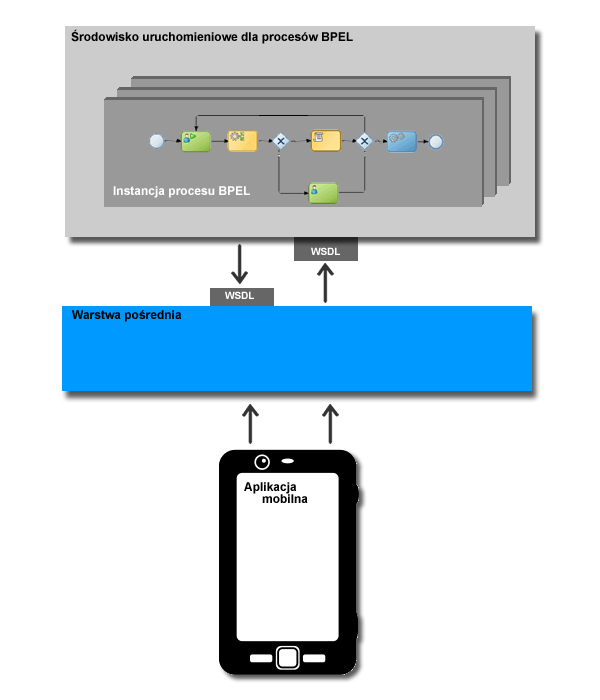
\includegraphics[scale=0.5]{middlewareConceptDiagram}}
\caption{Poglądowy schemat działania warstwy pośredniej}
\label{fig:middlewareConceptDiagram}
\end{figure}

Na rysunku~\ref{fig:middlewareConceptDiagram}. przedstawiono poglądowy schemat działania opisanego powyżej rozwiązania. Diagram ma na celu lepsze zobrazowanie problemu i wyłonienie funkcjonalności, które warstwa pośrednia musi realizować. Na schemacie można dostrzec trzy rodzaje systemów: środowisko uruchomieniowe dla procesów biznesowych, warstwę pośrednią oraz aplikację mobilną. Strzałki umieszczone na schemacie przedstawiają kierunki komunikacji pomiędzy poszczególnymi systemami.  Komunikacja między aplikacją mobilną a warstwą pośrednią zawsze odbywa się z inicjatywy aplikacji mobilnej, jest to związane ze specyfiką dostępu aplikacji do mediów komunikacyjnych. Wynika z tego, że jedną z funkcjonalności które musi  realizować warstwa pośrednia jest buforowanie żądań pochodzących z procesów biznesowych do momentu aż aplikacja mobilna się po nie zgłosi sama. 

Aplikacje mobilne są specyficzne pod jeszcze jednym względem - poszczególne instancje aplikacji uruchamiane są zawsze na urządzeniach personalnych. Bardzo mocny akcent zatem kładziony jest tutaj na samych użytkowników. Gdy przyglądniemy się procesowi BPEL to możemy dostrzec, że wątek ludzki jest w nich zupełnie pomijany. Proces komunikuje się z usługą sieciową jedynie w celu rozwiązania jakiegoś konkretnego zadania i zazwyczaj oczekuje na rezultat.

%---------------------------------------------------------------------------

\section{BPEL4People}
\label{sec:BPEL4People}

Jak wspomniano powyżej procesy WS-BPEL traktują użytkowników po macoszemu, skupiają się przede wszystkim na sekwencji wykonywania kolejnych operacji. Problem dostrzegli projektanci z zespołów IBM oraz SAP, a proponowaną przez nich odpowiedzią jest powstanie rozszerzenia do BPEL nazwanego \textit{BPEL4People}.  

Twórcy standardu argumentują powstanie kolejnej specyfikacji koniecznością uwzględnienia aspektu ludzkiego w procesach BPEL. Podają szereg przykładów, w których interakcja procesu z człowiekiem jest konieczna. Jednym z przykładów jest konieczność dokonywania decyzji akceptacji lub odrzucenia wyniku jakiejś operacji. Innym przykładem jest wprowadzanie dodatkowych danych niezbędnych do kontynuacji wykonania procesu, za pomocą formularzy. \cite[str. 4]{bpel4People}

Specyfikacja opiewa w szereg bardzo ciekawych pomysłów integracji interakcji użytkowników z  procesami BPEL. Porusza problem przejścia pomiędzy serwisami dostosowanymi dla ludzi a serwisami zautomatyzowanymi, zwraca uwagę na  problem monitorowania zadań przeznaczonych dla ludzi, opisuje problem terminów ostatecznych wykonania zadań oraz eskalacji w przypadku ich przekroczenia.\cite[str. 6]{bpel4People}

\subsection{WS-HumanTask}

Bezpośrednio powiązany  z rozszerzeniem BPEL4people jest temat usług sieciowych dla ludzi, które są wykorzystywane przez to rozszerzenie.

\textit{WS-HumanTask} są usługami sieciowymi 'implementowanymi' przez ludzi. Pozwalają na integrację ludzi z aplikacjami zorientowanymi na usługi (SOA). Specyfikacja udostępnia dwa interfejsy do komunikacjami z zadaniami. Pierwszy z nich jest przeznaczony dla automatów czyli aplikacji rozproszonych, drugi natomiast jest przeznaczony dla ludzi i pozwala na operacje zadaniami.  
Zadania opisane w specyfikacji posiadają przypisania do konkretnych grup docelowych. Przypisania te definiują kto powinien być uprawniony do operacji na zadaniach. Specyfikacja definiuje również meta dane dotyczące zadań, pozwalające na określenie w jaki sposób zadania mają być prezentowane na różnych urządzeniach. Zadanie mogą również definiować reakcje na terminy ostateczne ich wykonania, w postaci mechanizmu eskalacji. 

\subsection{Implementacje}

Z punku widzenia proponowanego w niniejszej pracy magisterskiej rozwiązanie zastosowanie BPEL4People rozwiązuje szereg problemów związanych ze spersonalizowaną specyfiką aplikacji mobilnych. Kolejne instancje aplikacji mobilnych można utożsami z użytkownikami. Warstwa pośrednia udostępniałaby w takim podejściu WS-HT, z którymi komunikowałby się proces \textit{BPEL4People}. Niestety rzeczywistość w tym przypadku okazuje się brutalna. Rozszerzenie do BPEL jeśli nie zostaje zaimplementowane jest bezwartościowe. W przypadku BPEL4People mimo tego że standard istnieje już 9 lat, nie został jeszcze wdrożony w żadnym z popularnych środowisk uruchomieniowych.  
Warstwa pośrednia powinna więc, samodzielnie uwzględniać aspekt ludzki pomijany przez procesy WS-BPEL. 

Mimo braku implementacji można dostrzec pewne korzyści płynące z powstania rozszerzenia BPEL4People. Są nimi z pewnością pomysły dotyczące rozwiązania problemu dystrybucji żądań pochodzących z procesów WS-BPEL między różnymi użytkownikami. W niniejszej pracy magisterskiej niejednokrotnie skorzystamy z tej wiedzy. 

%---------------------------------------------------------------------------

\section{Zadania}
\label{sec:tasks}

Pierwszym z pomysłów zaczerpniętych z \textit{BPEL4People} jest pomysł na traktowanie kolejnych żądań pochodzących z procesów WS-BPEL jako zadań, a aplikacji mobilnych jako zespołu specjalistów potrafiących rozwiązać te zadania. Podejście to rozwiązuje problem konieczności buforowania żądań procesu ze względu na komunikacje pull od strony aplikacji mobilnej. 

\begin{figure}[h]
\centerline{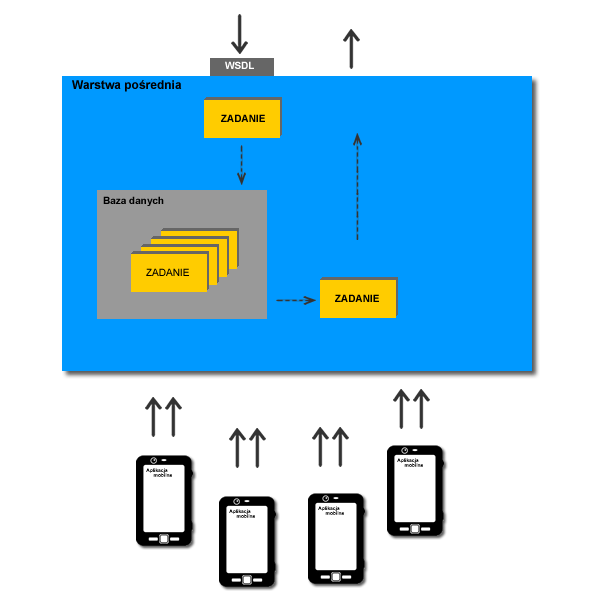
\includegraphics[scale=0.5]{middlewareTasksConceptDiagram}}
\caption{Poglądowy schemat wykorzystania zadań w warstwie pośredniej.}
\label{fig:middlewareTasksConceptDiagram}
\end{figure}

Na rysunku~\ref{fig:middlewareTasksConceptDiagram}. przedstawiono poglądowy schemat wykorzystania zadań w warstwie pośredniej. Strzałkami przerywanymi został oznaczony podstawowy cykl życia zadania. Po otrzymaniu żądanie od procesu BPEL warstwa pośrednia utworzy nowe zadanie i zapisze go w bazie danych. Aplikacje mobilne korzystając z lekkiego interfejsu komunikacyjnego, będą potrafiły pobierać zadania z bazy danych w celu ich rozwiązania. Po rozwiązaniu zadania, następować będzie wysłanie odpowiedzi do procesu biznesowego. 

\subsection{Dystrybucja zadań}
Przedstawiony powyżej schemat nie jest jednak kompletny. Oczywistym jest, że aby proces biznesowy miał sens powinien wykonywać więcej niż jedną operację, dla każdej operacji w proponowanym rozwiązaniu istnieć będzie zupełnie inna klasa zadań. Nie trudno dojść do wniosku, że każda z tych klas obsługiwana może być przez zupełnie różne grupy użytkowników. Na przykład niemal w każdym przedsiębiorstwie zadania dyrektora są kompletnie inne od zadań zwykłego pracownika, ale są one między sobą w jakiś sposób powiązane na przykład występują w tym samym procesie. Wnioskiem z tego płynącym jest konieczność wprowadzenia w warstwie pośredniej mechanizmu przydzielania zadań poszczególnym użytkownikom. W przypadku tym ponownie rozszerzenie \textit{BPEL4People} przewidziało ten problem i zaproponowało rozwiązanie. Wprowadza ono do każdej klasy zadań, definicje grupy docelowych adresatów. 

\begin{figure}[h]
\centerline{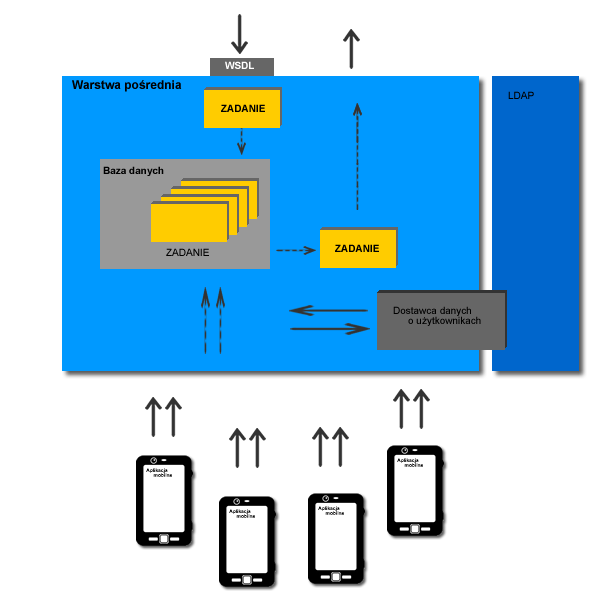
\includegraphics[scale=0.5]{middlewareUserDataProviderConceptDiagram}}
\caption{Schemat warstwy pośredniej uzupełniony o zarządzanie użytkownikami.}
\label{fig:middlewareUserDataProviderConceptDiagram}
\end{figure}

Na rysunku ~\ref{fig:middlewareUserDataProviderConceptDiagram} przedstawiono schemat warstwy pośredniej uzupełniony o zarządzanie użytkownikami. Aplikacje mobilne podczas rozwiązywania zadań będą przedstawiać się przy pomocy nazwy użytkownika. Przed pobraniem zadań z bazy danych dostawca danych o użytkownikach dostarczy informacji niezbędnych do określenia zadań specyficznych dla danego użytkownika. Sposób ten zapewni, że zadania należące do dyrektora przedsiębiorstwa nie trafią do zwykłych pracowników. 

Zastosowanie dodatkowej warstwy nazwanej \textit{Dostawcą danych o użytkownikach} jest tutaj celowe, i będzie wymagać osobnej implementacji dla różnych rodzajów metod przechowywania danych o użytkownikach. Nie koniecznie użytkownicy musza pochodzi z systemu katalogowego takiego jak LDAP. Możliwości przechowywania danych o użytkownikach jest bardzo wiele, dla prostych systemów lista użytkowników może być nawet predefiniowana.

\subsubsection{Context aware middleware}
Dodatkowym atutem udostępnienia możliwości implementacji dostawcy jest możliwość integracji adaptera z systemami zwanymi \textit{Context aware middleware}. 

\textit{Context aware middleware} jest oprogramowaniem które za pomocą danych dostarczanych z możliwie jak największej ilości źródł, stara się rozwiązać zadany problem. Rozwiązanie to bardzo szerokie zastosowanie znajduje głównie w aplikacjach mobilnych, dlatego że kontekst w przypadku tych aplikacji zmienia się bardzo dynamicznie. Architektura skupia się przede wszystkim na dostarczeniu informacji opisujących takie wymiary jak: - miejsce, Gdzie ? - czas, Kiedy? - stan np. Jaka jest temperatura otoczenia? - podmiot, Kto?

Bazując na tych danych stara się rozwiązywać dany problem w najbardziej optymalny sposób, na przykład przydzielając zadania osobie która jest najbliżej, która jest najmniej obciążona, która jest aktualnie w pracy itd.

Aby zastosować \textit{Context aware middleware} w warstwie pośredniej wystarczy odpowiednia implementacja dostawcy danych o użytkownikach. Uzyskamy dzięki takiemu rozwiązaniu potężne narzędzie potrafiące dystrybuować zadania w bardzo optymalny sposób zapewniając ich szybką realizację.  

\subsection{REST API}

Interfejs komunikacji warstwy pośredniej od strony procesów biznesowych został wymuszony przez specyfikację BPEL. Aby skompletować projekt warstwy pośredniej konieczne jest zdefiniowanie interfejsu komunikacyjnego od strony aplikacji mobilnych. 

Interfejs ten powinien przede wszystkim rozwiązywać podstawowy problem, występujący podczas rozwiązywania zadań przez wielu użytkowników jakim są konflikty. Nie może on dopuścić do sytuacji w której jedno zadanie byłoby rozwiązywanie przez wielu użytkowników jednocześnie. W celu rozwiązanie tego problemu konieczne jest wprowadzenie statusów zadań. W proponowanej warstwie pośredniej będą występowały następujące statusy zadania:

\begin{itemize}
\item gotowe do wykonania (ang. ready) -- zadanie zostanie oznaczone tym statusem tuż po utworzeniu. Użytkownik aplikacji mobilnych szukając zadań do wykonania otrzyma listę zadań oznaczonych właśnie tym statusem. 
\item przypisane (ang. climed) -- status ten oznacza, że któryś z użytkowników zadeklarował chęć jego wykonania. Będzie ono od tej pory dostępne tylko dla tego użytkownika. Pozostali użytkownicy poszukujący zadań do wykonania go nie zobaczą. 
\item rozwiązane (ang. completed) -- statusem tym oznaczone będą zadania zrealizowane z sukcesem, których rezultat został odesłany do procesu biznesowego. 
\item błąd podczas rozwiązywania (ang. failed) -- statusem tym oznaczone zostaną wszystkie zadania, podczas których rozwiązania wystąpił problem techniczny. 
\end{itemize}

Znając poszczególne statusy nadszedł czas na określenie interfejsu komunikacyjnego z aplikacjami mobilnymi. Ponieważ wśród aplikacji mobilnych najbardziej popularnym medium komunikacyjnym jest połączenie sieciowe na pewno najrozsądniejszym pomysłem będzie z niego skorzystanie. Jak wspomniano w rozdziale ~\ref{cha:analizaAplikacjiMobilnych}, podczas projektowania aplikacji mobilnych należy zwrócić uwagę na to aby wybierane technologie nie obciążały zbytnio ograniczonego pod względem zasobów urządzenia mobilnego. Dobrym wyborem w takim wypadku będzie REST. 

\subsubsection{Usługi sieciowe RESTFul}

REST (ang. Representational State Transfer) jest wzorcem narzucającym dobre praktyki tworzenia architektury aplikacji rozproszonych. Usługi sieciowe RESTFul  są usługami zaimplementowanymi na bazie protokołu HTTP i głównych zasad REST. ~\cite{rest}
Podstawą architektury REST jest zasób, zasób jest tutaj traktowany nie tylko jako jakiś byt, który można pobrać z aplikacji internetowej za pomocą protokołu HTTP. Zasobem w architekturze REST są również usługi udostępniane przez aplikacje internetowe.  

Kolejnym z głównych założeń architektury REST jest wykorzystanie metod udostępnianych przez protokół HTTP do definicji operacji wykonywanych na danym zasobie. Protokół HTTP oprócz najbardziej popularnych metod jak GET i POST udostępnia również całą gamę pozostałych metod. W architekturze REST oprócz tych dwóch najpopularniejszych bardzo często wykorzystywane są również PUT oraz DELETE. Znaczenie poszczególnych metod w kontekście operacji na zasobie może przedstawiać się następująco:
\begin{itemize}
\item GET -- pobranie danych
\item POST -- dodawanie danych
\item PUT -- edycja danych
\item DELETE -- usuwanie danych 
\end{itemize}


\subsubsection{Definicja interfejsu}

Warstwa pośrednia do komunikacji z aplikacjami mobilnymi będzie udostępniać następujące funkcje:

\begin{itemize}
\item lista zadań do wykonania -- metoda nie będzie przyjmować żadnych parametrów dodatkowych, kontekst użytkownika zostanie określony na podstawie nagłówków http wymaganych przez HTTP Basic Authentication. 
\item przypisz do zadania -- metoda jako parametr będzie przyjmować unikalny identyfikator zadania  
\item zrezygnuj z zadania -- metoda jako parametr będzie przyjmować unikalny identyfikator zadania  
\item rozwiąż zadanie -- metoda jako parametr będzie przyjmować unikalny identyfikator zadania  oraz wynik rozwiązania zadania. 
\end{itemize}

%---------------------------------------------------------------------------

\section{Wybrane technologie}
\label{sec:technologies}

Niemal w każdym projekcie informatycznym kluczową sprawą jest dobór odpowiednich technologii. Do realizacji warstwy pośredniej potrzebna będzie technologia webowa potrafiąca udostępnić usługi sieciowe, potrafiąca komunikować się z bazą danych i posiadająca wsparcie dla technologii REST. Niemal wszystkie popularne języki programowania spełniają każdy z tych warunków. Należy zatem pójść o jeden krok dalej i poszukać gotowego frameworka (zestawu gotowych bibliotek i wzorców postępowania), który przy wykorzystaniu jednego z tych języków będzie potrafił zrealizować przynajmniej cześć zadań. Wybór w niniejszej pracy magisterskiej padł na Spring Framework zaimplementowany w języku Java. 

\subsection{Spring Framework  }
Spring Framework zapewnia kompleksowy model programistyczny i konfiguracyjny dla nowoczesnych aplikacji biznesowych opartych na języku Java. Kluczowym elementem jest wsparcie infrastrukturalne  na poziomie aplikacji: Spring skupia się na "hydraulice" aplikacji dla przedsiębiorstw, tak, że zespoły mogą skupić się na logice biznesowej na poziomie aplikacji, bez konieczności określania środowisk programowania. ~\cite{springFramework}

\begin{itemize}

\item Spring Web Services  -- w przypadku warstwy pośredniej jedną z głównych funkcjonalności koniecznych do realizacji jest udostępnienie usług sieciowych do komunikacji z procesami biznesowymi. Spring Framework posiada specjalnie do tego celu przygotowany moduł nazwany Spring Web Services. Moduł ten koncentruje się tworzeniu usług sieciowych na podstawie dokumentów SOAP przy wykorzystaniu stylu, umowa-najpierw(ang. contract-first). Styl ten polega na definicji interfejsów w postaci plików WSDL, przed stworzeniem konkretnej implementacji usługi. Jak argumentuje Spring styl ten pozwala na tworzenie elastycznych usług sieciowych przy wykorzystaniu jednego z wielu sposobów na manipulacje zawartością XML.  ~\cite{springWS}

\item Spring MVC -- moduł MVC jak sama nazwa wskazuje jest przeznaczony do tworzenia aplikacji opartych o jeden z najbardziej popularnych wzorców projektowych Model Widok Kontroler. Spring MVC jest przeznaczony przede wszystkim do zastosowania wzorca w aplikacjach webowych gdzie do komunikacji wykorzystywany jest protokół HTTP. W przypadku aplikacji webowych widokiem zazwyczaj jest dynamicznie generowany kod HML, nie jest to jednak reguła. W przypadku warstwy pośredniej MVC zostanie wykorzystane do przygotowania REST API. Widokiem w takim wypadku będą dane opisane za pomocą dokumentów JSON. 

\item Spring Data -- Oprócz wyżej wymienionych modułów, Spring Framework dostarcza również wsparcie do obsługi komunikacji z bazą danych, najczęściej do tego celu wykorzystując popularne ORM'y ( Biblioteki do mapowania obiektowo relacyjnego) jak Hibernate. W przypadku warstwy pośredniej istnieje konieczność przechowywania zadań w bazie danych dlatego Spring Data również zostanie wykorzystany.

\item Spring Secutiry -- W niniejszym rozwiązaniu uwierzytelnienia użytkowników REST API będzie odbywało się za pomocą HTTP Basic Authentication. Spring posiada również dodatkowe wsparcie do obsługi bezpieczeństwa przy pomocy HTTP Basic Authentication, wsparcie to udostępnione jest za pomocą modułu Spring Security.   

\end{itemize}

\subsection{MongoDB}

Bardzo ważną decyzją jest również wybór odpowiedniej bazy danych. Wymagania dotyczące warstwy pośredniej jasno określają, że głównym modelem przechowywanym w bazie danych będzie zadanie. Zadanie oprócz podstawowych informacji takich jak identyfikator, status, data utworzenia itd. będzie posiadał wszelkie informacje potrzebne do jego utworzenia, oraz jeśli zadanie zostanie wykonane posiadać będzie również informacje o rozwiązaniu. W przypadku skorzystania z relacyjnej bazy danych klaruje nam się przykładowy schemat bazy danych przedstawiony na rysunku ~\ref{fig:erd}.

\begin{figure}[h]
\centerline{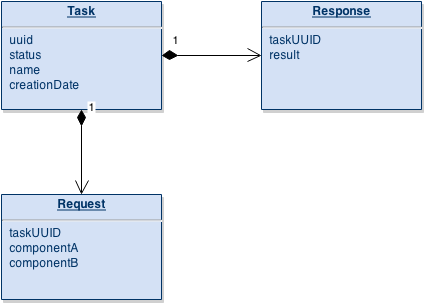
\includegraphics[scale=0.7]{erd}}
\caption{Diagram ERD przykładowego schematu bazy danych relacyjnej.}
\label{fig:erd}
\end{figure}

W przypadku pojedynczego zadania schemat może okazać się słuszny, problem powstaje gdy warstwa pośrednia obsługuje więcej niż jedno zadanie. W takim przypadku każdy kolejny rodzaj danych wejściowych poszczególnych zadań powinien znajdować się w osobnej tabeli. Mało tego dane wejściowe zadań nie muszą ograniczać się jedynie do płaskiej struktury danych. Mogą one zawierać argumenty będące osobnymi strukturami danych. W takich przypadkach, z punktu widzenia normalizacji bazy danych, każda z tych struktur powinna również znajdować się w osobnych tabelach.  Taka postać rzeczy ma bardzo negatywny wpływ na poziom komplikacji zapytań wyciągających zadania dla poszczególnych użytkowników. Mogą istnieć przypadki w których na podstawie danych wejściowych będzie potrzeba ograniczenia adresatów zadania, np. wybrania użytkowników w obrębie kilku kilometrów od adresu znajdującego się w danych wejściowych. 

Sposobem na rozwiązanie problemu nie koniecznie płaskiej struktury danych wejściowych może być zastosowanie typu XML do przechowywania tych danych. W takich przypadkach dane wejściowe zostałyby serializowane do dokumentów xml i w takiej postaci zapisane w bazie danych. Kolejny raz problemem są jednak skomplikowane zapytania do bazy danych. 

Odpowiedzią na postawione wymagania są dokumentowe bazy danych. Przechowują one dane w postaci kolekcji dokumentów. Dokumenty przechowywane w bazie danych mogą posiadać dowolnie skomplikowaną strukturę danych, a odpowiednio przygotowane zapytania będą potrafiły filtrować  listę tych dokumentów na podstawie wszystkich argumentów znajdujących się w tej strukturze. 

Przykładowy dokument bazy danych MongoDB może przedstawiać się następująco:

\begin{lstlisting}[caption=Zadanie w postaci dokumentu MongoDB.,numbers=left]
{	
	uuid : '6942cd9b-3b3b-49bd-9b18-de68384bd22a',
	name : 'createWarehouseDocument',
	state : '',
	createDate : '2014-07-24',
	priority: 3,
	request : {
		document :{
			type: 'inbound',
			company : {
				name : 'AGH',
				address : {
					city: 'Krakow',
					streat : 'al. A. Mickiewicza',
					number: '30',
					country: 'Polska'
				}
			},
			positions: [...]
		}
	}
}
\end{lstlisting}


Przedstawiony wyżej dokument jest przykładem zadania którego celem jest stworzenie odpowiedniego dokumentu magazynowego. Możemy sobie wyobrazić sytuację, że dokumenty dla kontrahentów z poszczególnych krajów są tworzone przez różnych użytkowników. Przykładowe zapytanie znajdujące wszystkie zadania dla użytkownika obsługującego Polskę wyglądało by następująco. 

\begin{lstlisting}[caption=Zapytanie MongoDB.]
{'request.document.company.address.country': 'Polska'}
\end{lstlisting}

W przypadku relacyjnej bazy danych powyższa struktura wymagała by stworzenie sześciu tabel a zapytanie które dałby by dokładnie taki sam rezultat wyglądało by następująco:

\begin{lstlisting}[caption=Zapytanie SQL.]
SELECT * FROM Tasks t 
	JOIN Request r ON t.id = r.task_id
	JOIN Document d ON r.id = d.request_id
	JOIN Company c ON d.id = c.document_id
	JOIN Address a ON c.id = a.company_id
WHERE a.country = 'Polska';
\end{lstlisting}

\subsection{Maven}
Kolejna technologią wykorzystaną do realizacji idei przestawionej w niniejszej pracy magisterskiej jest Maven. Wykorzystanie tej technologii wynika z decyzji wykorzystania języka Java. Maven jest narzędziem wspomagającym budowanie projektów stworzonych w języku Java. Odpowiada on za skompletowania wszystkich wymaganych bibliotek zdefiniowanych w odpowiednim pliku konfiguracyjnym - pom.xml. Biblioteki te pobierane są ze specjalnie przygotowanych do tego celu repozytoriów dostępnych w sieci, na lokalną maszynę. Biblioteki te są następnie wykorzystywane w procesie budowania plików wynikowych.  

%---------------------------------------------------------------------------

\section{Sprawienie rozwiązania generycznym}
\label{sec:generic}

Przedstawiony do tej pory model warstwy pośredniej skupia się przede wszystkim na problemie komunikacji pomiędzy procesem biznesowym oraz aplikacją mobilną, opisuje również sposób przechowywania i dystrybucji zadań. Model jest przy okazji bardzo ogólny i możliwy do zastosowania bez względu, na rozwiązywany problem. Nie ma w nim mowy o konkretnych przypadkach zastosowań. 

Dobrym pomysłem będzie więc stworzenie rozwiązania na tyle elastycznego aby mogło być wykorzystywane bez względu na rozwiązywany problem. W środowisku IT taki model postępowanie nazywany jest generycznym. W przypadku warstwy pośredniej sposób zarządzania zadaniami jest taki sam dla wszystkich rodzajów zadań - utworzenie zadania po otrzymaniu żądania od procesu, udostępnienie zadania aplikacją mobilnym, odpowiedź do procesu. Główną różnicą są dane wejściowe różnych żądań oraz sposób dystrybucji zadań pomiędzy aplikacjami na podstawie tych danych. Problem różnych struktur danych wejściowych dla różnych zadań rozwiązuje nam wybór bazy danych MognoDB, który będzie potrafił zapisać te struktury bez dodatkowych konfiguracji, oraz będzie potrafił je przeszukiwać za pomocą prostych zapytań. 

Problem różnego sposobu dystrybucji danych rozwiążemy za pomocą pliku konfiguracyjnego, który będzie opisywał poszczególne zadania, oraz definiował jakie grupy użytkowników są uprawnione do ich rozwiązywania.

Opisany model można zobrazować za pomocą schematu widocznego na rysunku ~\ref{fig:middlewareGenericConcept}.

\begin{figure}[h]
\centerline{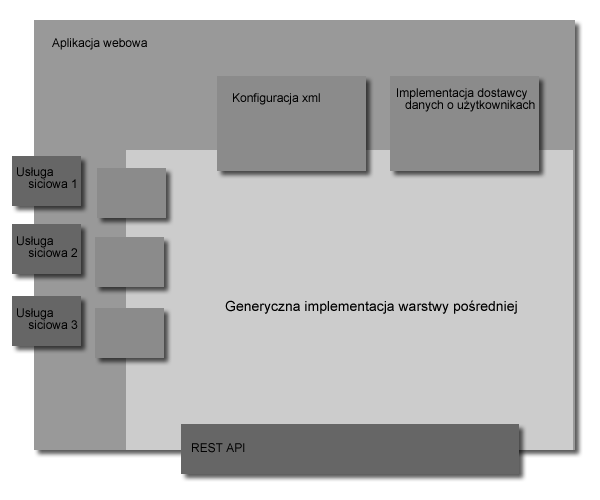
\includegraphics[scale=0.6]{middlewareGenericConcept}}
\caption{Poglądowy schemat wydzielenia biblioteki odpowiedzialnej za obsługę warstwy pośredniej.}
\label{fig:middlewareGenericConcept}
\end{figure}

Podsumowując, opisane w niniejszej pracy magisterskiej rozwiązanie będzie generyczną biblioteka służącą do tworzenie aplikacji webowej. Aplikacja ta będzie warstwa pośrednią pomiędzy procesem biznesowym a aplikacjami mobilnymi. 

%---------------------------------------------------------------------------

\section{Implementacja}
\label{sec:impl}

Implementacja biblioteki zostanie przedstawiona w sposób schematyczny, zostanie przedstawiony projekt klas występujących w rozwiązaniu wraz z ich opisem. W następnej część zostaną przedstawione diagramy sekwencji najważniejszych funkcjonalności rozwiązania, opisujące przebieg wywołań kolejnych funkcji zdefiniowanych klas. 

\subsection{Diagram klas}

\begin{figure}[h]
\centerline{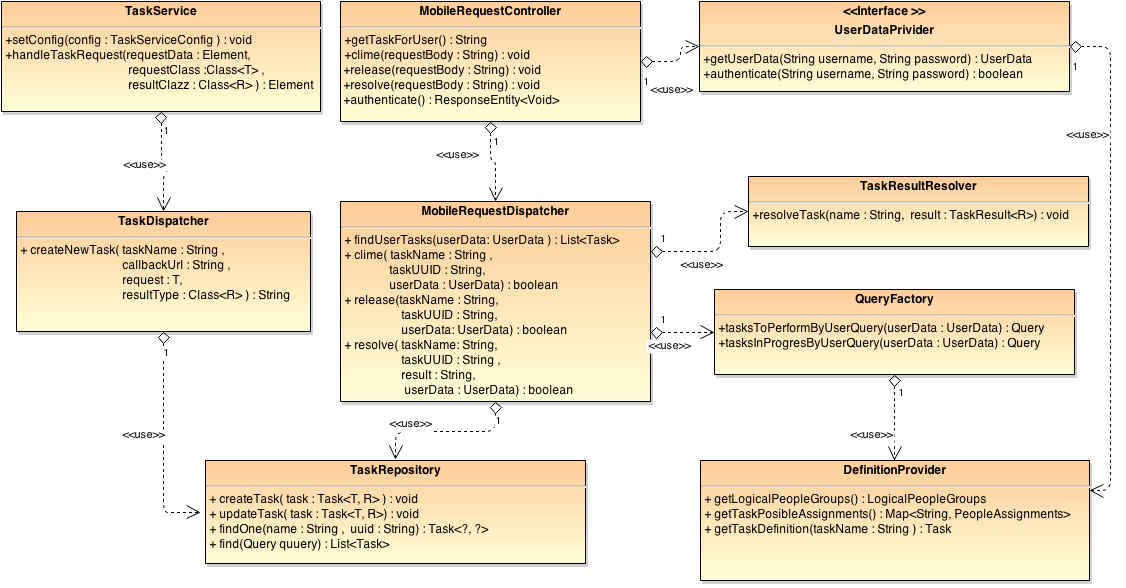
\includegraphics[scale=0.45]{classDiagram}}
\caption{Diagram klas implementacji warstwy pośredniej.}
\label{fig:classDiagram}
\end{figure}

Diagram klas przedstawiony na rysunku~\ref{fig:classDiagram}. przedstawia zestaw klas, które wymagają dodatkowego objaśnienia: 


\begin{itemize}
\item TaskService -- jest to klasa odpowiedzialna za obsługę żądań pochodzących z procesów biznesowych. Każdy rodzaj zadania powinien posiadać własną instancję tej klasy, która z kolei powinna być wykorzystywana przez usługę sieciową odpowiedzialną za jego obsługę. Klasa posiada dwie metody, setConfig odpowiedzialną za ustawienie podstawowych informacji o zadaniu, które będzie obsługiwać instancja tej klasy, takich jak nazwa, lista klas definiujących dane wejściowe i wyjściowe zadania. Kolejną metodą jest metoda handleTaskRequest metoda ta przyjmuje jako parametr obiekt typu Element zawierający dane wejściowe w postaci XML. Metoda przetwarza te dane na odpowiednie klasy i zapisuje zadanie w bazie danych do późniejszej realizacji. Zwraca ona obiekt typu Element zawierający informacje o unikalnym identyfikatorze przypisanym zadaniu, obiekt ten jest plikiem xml który powinna zwrócić usługa sieciowa. Metoda handleTaskRequest powinna zostać wywołana przez usługę sieciową odbierającą żądanie od procesu biznesowego.
\item TaskDispatcher -- Klasa odpowiedzialna za przetwarzanie, przyjętych przez klasę TaskService zadań. Posiada ona jedną metoda służącą do zapisu zadania przetworzonego przez  TaskService, nazwaną createNewTask.
\item TaskRepository -- repozytorium zadań odpowiedzialne za obsługę bazy danych. Posiada metody służące do zapisu i edycji zadań oraz do wyszukiwania zarówno pojedynczych zadań, jak i ich listy. 
\item MobileRequestController -- klasa przeznaczona do udostępnienia REST API. Posiada ona metody udostępniane przez interfejs przeznaczony do aplikacji mobilnych. Klasa ta korzystając ze Spring Security, odnajduje kontekst aktualnego użytkownika, pobiera informacje o nim za pomocą UserDataProvidera przekazując następnie kontrole MobileRequestPrivider'owi. 
\item UserDataProvider -- interfejs służący do określenia metod które musi implementować dostawca informacji o użytkowniku. Implementacje UserDataProvidera będą wykorzystywana między innymi przez Spring Security.
\item DefinitionProvider -- klasa to odpowiedzialna jest za deserializację pliku xml zawierającego konfiguracje poszczególnych zadań, oraz dostarczenie tej konfiguracji do pozostałych klas warstwy pośredniej. 
\item MobileRequestDispatcher -- klasa odpowiedzialna za obsługę żądaniami pochodzącymi z aplikacji mobilnych. Współpracuje z klasami przeznaczonymi do generowania zapytań, wyciągania danych z bazy oraz odpowiedzialnymi za odesłanie rozwiązania do procesów biznesowych. 
\item QueryFactory -- głównym zadaniem tej klasy jest przygotowanie zapytań pozwalających odnaleźć zadania dostępne dla danego użytkownika. Zapytania generowane są na podstawie konfiguracji xml oraz danych o użytkowniku. 
\item TaskResultResolver -- klasa posiada tylko jedną metodę nazwaną resolveTask służąca do wysłania odpowiedzi do procesu biznesowego zawierającej rezultat wykonania zadania. 
\end{itemize}

\subsection{Diagramy sekwencji}

Sposób działania powyżej opisanych klas zostanie przedstawiony za pomocą diagramów sekwencji. Diagramy przedstawiają sekwencje kolejnych wywołań funkcji w celu realizacji funkcjonalności dostarczanych przez warstwę pośrednią. 

\begin{figure}[h]
\centerline{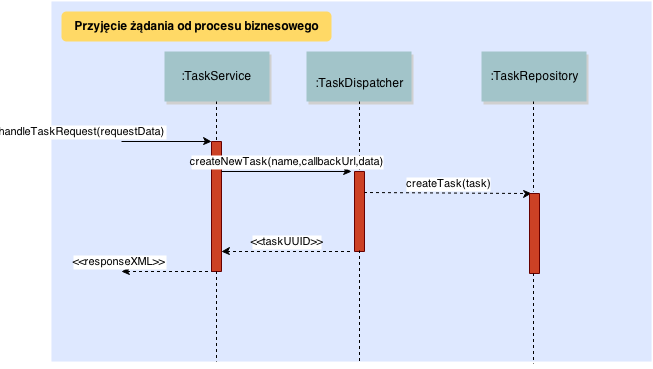
\includegraphics[scale=0.6]{createTaskFlow}}
\caption{Diagram sekwencji obsługi żądania pochodzącego z procesu BPEL.}
\label{fig:createTaskFlow}
\end{figure}

Na rysunku~\ref{fig:createTaskFlow} zobaczyć można diagram sekwencji funkcjonalności -przyjęcie żądania od procesu biznesowego. Usługa sieciowa korzystając z konkretnej instancji klasy TaskService uruchamia metodę handleTaskRequest przekazując do niej obiekt zawierający dokument XML z danymi wejściowymi. Wewnątrz metody, dokument XML zostaje zdeserializowany do postaci obiektów podanych w konfiguracji klasy TaskService. Zostaje również wydobyty adres url usługi przyjmującej ostateczny rezultat zadania. Sterowanie przekazywane jest następnie do klasy TaskDispatcher w celu utworzenie nowego zadania w bazie danych. Metoda createNewTask klasy TaskDispatcher oprócz stworzenia nowego dokumentu w kolekcji w bazie danych MongoDB za pomocą repozytorium TaskRepository, odpowiedzialna jest za generację unikalnego identyfikatora w postaci klucza GUID. Unikalny identyfikator jest następnie zwracany ponownie do TaskService'u gdzie zostaje opakowany w dokument XML, który zostanie zwrócony do procesu biznesowego. Wysłanie unikalnego klucza do procesu jest w tym przypadku krytyczne, po stronie silnika uruchomieniowego procesów biznesowych BPEL będzie istniało bardzo wiele instancji procesów w różnym stadium wykonania. Komunikacja procesu z warstwą pośrednią odbywa się w sposób asynchroniczny, poprzez kolejne wywołania aktywności request (wysłanie żądania), by następnie przejść do aktywności recieve (oczekiwać na jego rezultat). W między czasie proces może również wykonać inne operacje. Aby skojarzyć aktywność wysłania żądania z otrzymaniem żądania w przypadku wielu instancji procesu konieczna jest identyfikacja tych żądań za pomocą tego samego unikalnego klucza. W procesach biznesowych BPEL mechanizm ten został nazwanych mechanizmem korelacji.  Aby skorzystać zatem z mechanizmy korelacji, podczas tworzenia nowego zadania proces biznesowy musi otrzymać unikalny klucz tego zadania by następnie podczas otrzymania rezultatu zadania był w stanie skojarzyć ten rezultat z konkretną instancją procesu. Rezultat w takim wypadku również musi zostać podpisany unikalnym identyfikatorem zadania. 

\begin{figure}[h]
\centerline{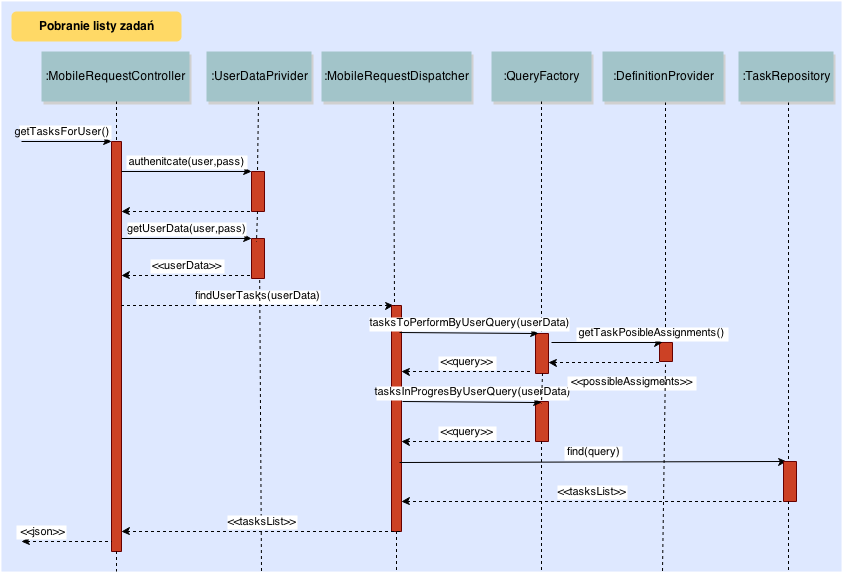
\includegraphics[scale=0.5]{tasksListFlow}}
\caption{Diagram sekwencji pobrania listy zadań dostępnych dla użytkownika.}
\label{fig:tasksListFlow}
\end{figure}

Rysunek~\ref{fig:tasksListFlow} przedstawia diagram sekwencji pobierania listy zadań przez aplikację mobilną. Sekwencja w tym przypadku zaczyna się od klasy MobileRequestController, która jest odpowiedzialna za obsługę żądań odpowiednich żądań http. Kontroler ten rozpoczyna wykonanie metody od autentykacji użytkownika którym przedstawia się żądanie http (z wykorzystaniem http basic authentication). Po poprawnej autentykacji zostają pobrane informacje o aktualnym użytkowniku, informacje te zostaną wykorzystane do wygenerowania listy zadań dla niego dostępnych.  Sterowanie zostaje następnie przekazane do klasy MobileRequestDispatcher, która za pomocą QueryFactory zbuduje dwa zapytania, jedno do wyciągnięcia nowych zadań do których użytkownika ma dostęp. Drugie zapytanie pokryje wszystkie zadania w trakcie realizacji przypisane do użytkownika. Zapytania te posłużą następnie do wyciągnięcia listy zadań z bazy danych przy pomocy repozytorium TaskRepository. Ostatnim krokiem będzie serializacja wydobytych zadań do postaci dokumentu JSON. 

\begin{figure}[h]
\centerline{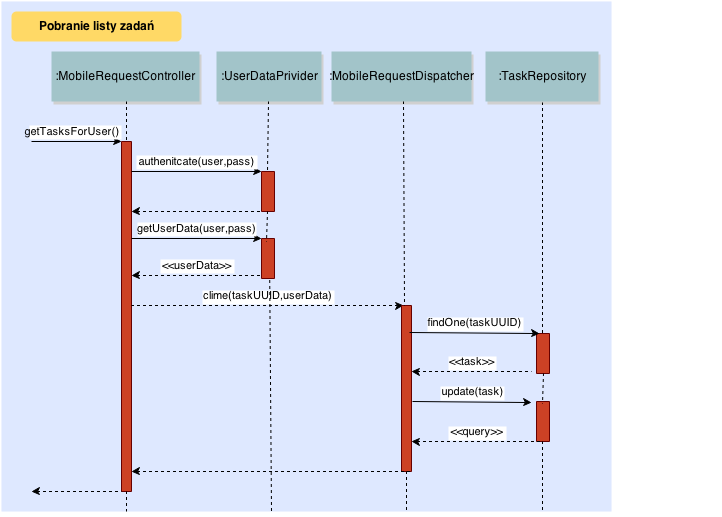
\includegraphics[scale=0.5]{climeTaskFlow}}
\caption{Diagram sekwencji przypisania użytkownika do zadania.}
\label{fig:climeTaskFlow}
\end{figure}

Rysunek ~\ref{fig:climeTaskFlow} przedstawia diagram przypisania konkretnego zadania do użytkownika. Przypisanie odbywa się za pomocą REST API. Odpowiednie żądanie HTTP zostaje przyjęte przez MobileRequestController, ponownie jak w przypadku pobierania listy zadań, dwie pierwsze operacje wykonywane przez kontroler to autentykacja i pobranie informacji o użytkowniku. Sterowanie zostaje następnie przekazane do MobileRquestDispatcher'a, który znajduje odpowiednie zadanie w repozytorium, zmienia jego status uzupełniając informacje o przypisanym użytkowniku by następnie zapisać te zmiany. Operacją kompensacyjną do przypisania jest operacja zwolnienia zadania. Diagram sekwencji w przypadku tej drugiej wygląda niemal identycznie jak diagram przypisania z tym że MobileRequrestDispatcher przywraca zadaniu status do realizacji. 

\begin{figure}[h]
\centerline{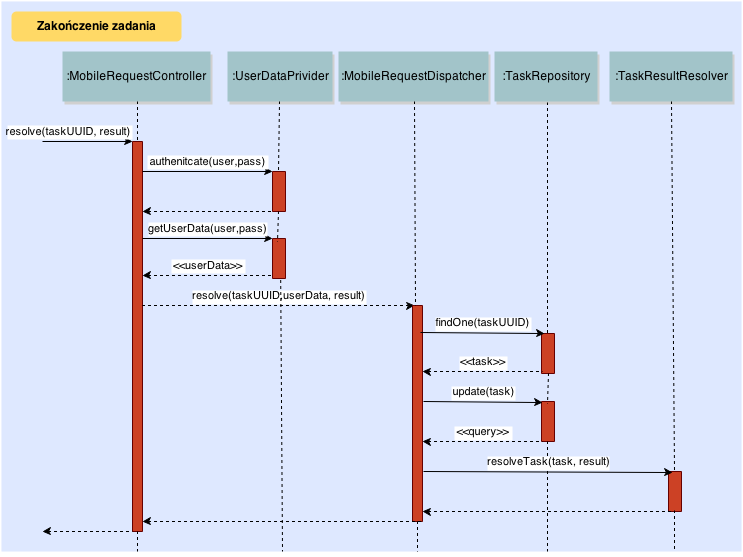
\includegraphics[scale=0.5]{resolveTaskFlow}}
\caption{Diagram sekwencji rozwiązania zadania.}
\label{fig:resolveTaskFlow}
\end{figure}

Na rysunku ~\ref{fig:resolveTaskFlow} przedstawiono ostatni rodzaj funkcjonalności jakim jest obsługa rozwiązania zadania. Decyzja o rozwiązaniu również pochodzi od strony aplikacji mobilnej i a funkcjonalność ją obsługująca udostępniona jest za pomocą REST API. Tak jak w poprzednich przypadkach przed rozpoczęciem przetwarzania żądania następuje autentykacja oraz pobranie informacji o użytkowniku. Następnie pobierane zostaje zadanie z repozytorium, ustawiany rezultat oraz zmieniany status. Rezultat następnie zostaje odesłany do procesu biznesowego przez klasę TaskResultResolver. Jeśli odesłanie rezultatu zakończy się sukcesem zadanie z odpowiednio ustawionym statusem i rezultatem zostaje zapisane do bazy danych.


%---------------------------------------------------------------------------

%\section{Notyfikacje}
%\label{sec:notifications}

%// TODO

\chapter{Warstwa pośrednia w zastosowaniu }
\label{cha:example}

Najlepszym sposobem weryfikacji każdego rozwiązania jest jego konfrontacja z rzeczywistością, przez znalezienie realnych przykładów jego użycia. Nie inaczej jest w przypadku proponowanego w niniejszej pracy rozwiązania. 

Pomysłem na przykład jest w tym przypadku proces sprzątania pokoju hotelowego. Celem przykładu jest zademonstrowanie działania warstwy pośredniej do komunikacji procesu biznesowego z aplikacjami mobilnymi, ale również pokazania sposobu integracji takiego rozwiązania z gotowymi systemami zewnętrznymi. 

%---------------------------------------------------------------------------

\section{Przedstawienie koncepcji}
\label{sec:concept}

Prezentacja przykładu zostanie rozpoczęta od przedstawienia koncepcji rozwiązania w postaci diagramów zaprojektowany za pomocą BPMN 2.0. Przedstawione zostaną dwa diagramy z których pierwszy jest sytuacją w której rozpoczyna się właściwy proces sprzątania hotelu. 

\begin{figure}[h]
\centerline{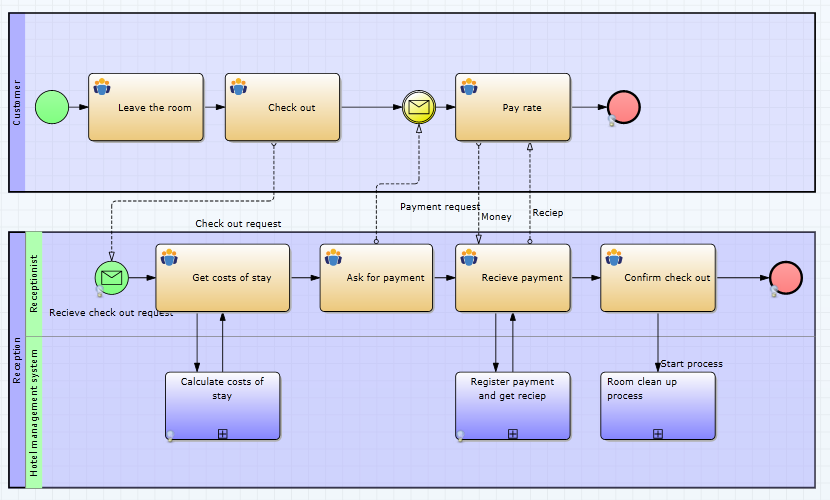
\includegraphics[scale=0.4]{hotelCheckOutProcess}}
\caption{Diagram BPMN procesu wymeldowania klienta z pokoju hotelowego.}
\label{fig:hotelCheckOutProcess}
\end{figure}

Na rysunku ~\ref{fig:hotelCheckOutProcess}, przedstawiono proces wymeldowania gościa hotelowego z pokoju po zakończonym pobycie. Klient hotelu po opuszczeniu pokoju udaje się do recepcji w celu oddania kluczy i uregulowania płatności. W recepcji przebywa recepcjonista, który odpowiedzialny jest za kontakt z klientem, o otrzymaniu kluczy prosi klienta o zapłatę kosztów pobytu. Po wymianie płatności na rachunek klient hotelowy opuszcza hotel, a recepcjonista oznacza pokój hotelowy jako gotowy do posprzątania, rozpoczynając w ten sposób właściwy proces. 

\begin{figure}[h]
\centerline{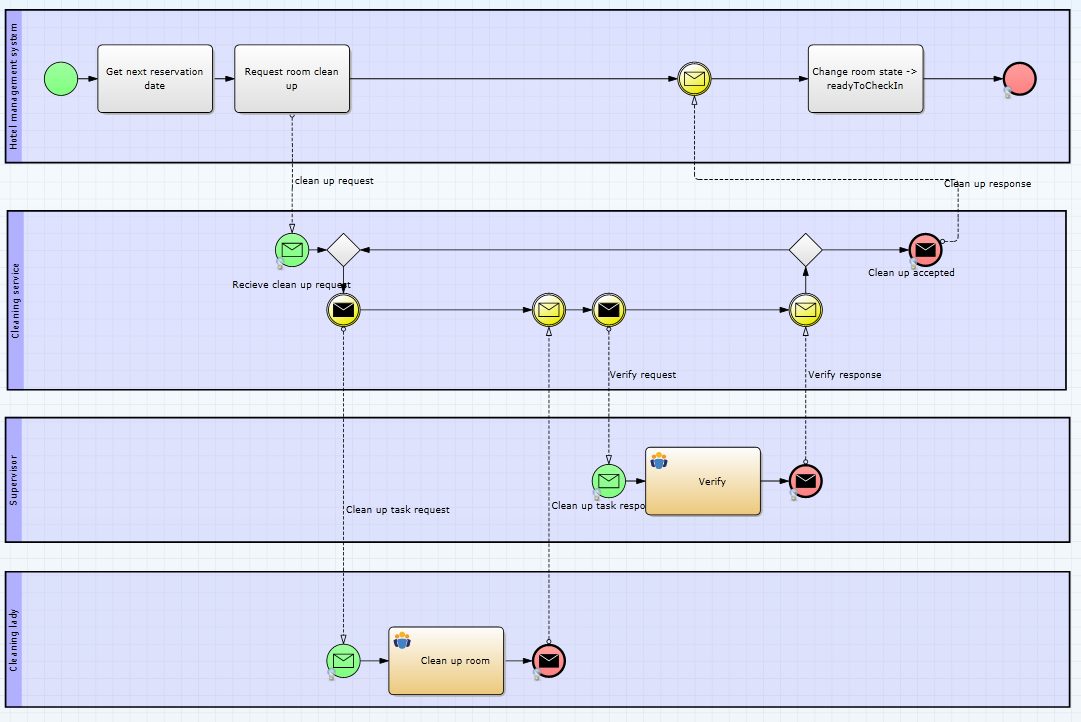
\includegraphics[scale=0.4]{roomCleanUpProcess}}
\caption{Diagram BPMN procesu sprzątania pokoju hotelowego.}
\label{fig:roomCleanUpProcess}
\end{figure}

Rysunek~\ref{fig:roomCleanUpProcess} przedstawia właściwy proces sprzątania pokoju hotelowego, widzimy na nim cztery rodzaje aktorów, każdy z nich oznaczony własną linią. Pierwszym z aktorów jest system zarządzania hotelem, jest to miejsce w którym recepcjonista oznacza pokój do posprzątania. System zarządzania hotelem jest miejscem w którym rozpoczyna się proces. Odpowiedzialny jest on za zebranie danych koniecznych do przeprowadzenia sprzątania a następnie przekazanie tych danych do kolejnego aktora, którym jest Serwis Sprzątający. A przypadku realizacji przykładu za pomocą opisanych w niniejszej pracy magisterskiej technologii aktora tego można utożsamić z procesem BPEL wraz z warstwą pośrednią. Serwis sprzątający odpowiedzialny jest za przeprowadzenie procesu sprzątania. Proces ten odbywa się przez wysłanie żądania do sprzątaczki (aplikacja mobilna), by po potwierdzeniu posprzątania pokoju wysłać żądanie do nadzorcy (również aplikacja mobilna) który będzie odpowiedzialny za weryfikacje sprzątania.  W przypadku braku akceptacji sprzątania przez nadzorcę pokój będzie musiał być kolejny raz posprzątany. W momencie zatwierdzenia sprzątania, rezultat trafi ponownie do Systemu Zarządzania Hotelem, aby recepcjonista mógł zameldować kolejnych gości. 

Na podstawie opisanego powyżej przykładu wyłonić można następujące systemy, których implementacja zostanie dokładniej opisana w dalszej części pracy.

\begin{itemize}
\item System Zarządzania Hotelem -- Dla celów przykładu, System Zarządzania Hotelem będzie prosta aplikacją internetową odpowiedzialną za udostępnienie formularza dla recepcjonisty oraz wyświetlenie listy rezultatów wykonania procesu.   
\item Proces BPEL -- Będzie to proces zawierający kompletną logikę biznesową odpowiedzialną za przeprowadzenie i weryfikacje sprzątania pokoju hotelowego. Proces ten będzie komunikował się zarówno z warstwą pośrednią jak i z Systemem Zarządzania Hotelem. 
\item Warstwa pośrednia --  Aplikacja internetowa odpowiedzialna za obsługę komunikacji procesu biznesowego z aplikacjami mobilnymi. 
\item Aplikacja mobilna -- aplikacja przeznaczona zarówno dla sprzątaczek jak i dla nadzorców. Udostępniać będzie bardzo prosty interfejs użytkownika służący do wyświetlenia listy zadań oraz do ich przypisywania i rozwiązywania. 
\end{itemize}


%---------------------------------------------------------------------------

\section{System Zarządzania Hotelem }
\label{sec:hotelManagementSystem}

Zadaniem tej aplikacji jest udostępnienie części funkcjonalność Systemu Zarządzania Hotelem przeznaczonej do oznaczania pokoju hotelowego jako wymagającego posprzątania. Aplikacja udostępniać będzie formularz w którym recepcjonista będzie mógł zgłosić pokój do posprzątania. Formularz będzie gromadził taki dane jak numer pokoju, numer piętra oraz kategorię do której należy pokój. Po zatwierdzeniu formularza  dane z niego pochodzące trafią do procesu biznesowego oraz do bazy danych w celu monitorowania postępu procesu. Kiedy proces zakończy swoje działania aplikacja odbierze za pomocą odpowiedniej usługi sieciowej jego rezultat. Odebranie rezultatu skutkować będzie zmianą statusu pokoju. Aplikacja udostępniać będzie również listę pokoi wraz z ich statusami w postaci strony html. 

\subsection{Wybrane technologie}
Aplikacja zostanie zrealizowana przy wykorzystaniu technologii:

\begin{itemize}
\item język programowania Java
\item Spring MVC
\item  Bootstrap Framework -- jest to zbiór  klas css oraz biblioteka stworzona w języku JavaScript, służący do tworzenia interfejsu użytkownika przy pomocy zaawansowanych kontrolek html.
\item Maven
\item Spring Web Services
\item Spring Data oraz Hibernate - jeden z najbardziej popularnych narzędzi ORM, przeznaczonych na platformę Java. 
\item H2 in memory - baza danych której cykl życia jest równoznaczny z cyklem życia aplikacji. Jest ona tworzona podczas uruchamiana aplikacji, dane znajdujące w się w niej są przechowywane w pamięci podręcznej. Bazy tego typu wykorzystywane są przede wszystkim do implementacji testów jednostkowych. Zdecydowanym plusem skorzystania z tego rodzaju bazy danych jest brak konieczności instalacji dodatkowych narzędzi co w przypadku niniejszego przykładu jest dużym udogodnieniem. 
\end{itemize}

\subsection{Implementacja}

\begin{figure}[h]
\centerline{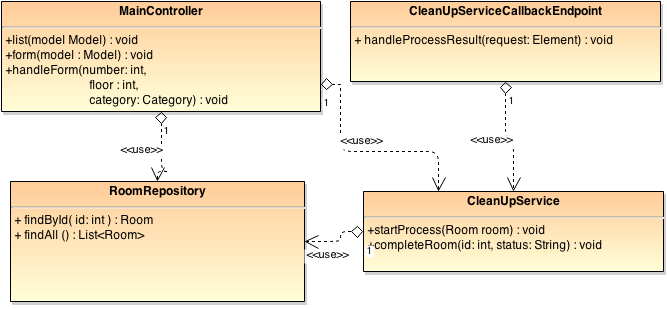
\includegraphics[scale=0.6]{hotelManagementSystemClasses}}
\caption{Diagram klas systemu zarządzania hotelem.}
\label{fig:hotelManagementSystemClasses}
\end{figure}


Na rysunku~\ref{fig:hotelManagementSystemClasses} został przedstawiony diagram klas Systemu Zarządzania Hotelem. Znajdują się na nim jedynie najbardziej istotne klasy z punku widzenia tej implementacji. Klasa MainController jest odpowiedzialna za udostępnienie interfejsu użytkownika oraz za obsługę żądań z niego pochodzących. Udostępnia ona trzy metody: 


\begin{itemize}
\item list -- metoda za pomocą RomRepository pobiera z bazy danych wszystkie pokoje, które zostały zgłoszone do posprzątania. Pobrana lista jest  następnie umieszczana w dynamicznej stronie html za pomocą technologii JSP. 
\item form -- metoda odpowiedzialna za wyświetlenie formularza w postaci html dla użytkownika. 
\item hadleForm -- metoda ta jest uruchamiana w przypadku zatwierdzenia danych wprowadzonych do formularza przez użytkownika. Metoda dodaje nowy pokój do bazy danych oraz uruchamia proces biznesowy z wykorzystaniem klasy CleanUpService. 
\end{itemize}

Druga bardzo ważną klasą jest CleanUpServiceCallbackEndpoint, jest to klasa stworzona z wykorzystaniem technologii Spring Web Services. Klasa ta obsługuje zdefiniowaną w konfiguracji usługę sieciową. Usługa służy do odbierania rezultatów wykonania procesu biznesowego. Jej rolą jest przeczytania komunikatu przysłanego przez proces biznesowy by następnie zmienić status sprzątanego pokoju za pomocą klasy CleanUpService. 

\subsection{Uruchomienie}

Aplikacja jest kompilowana do postaci pliku o rozszerzeniu war. Pliki tego typu mogą być uruchamiana na dowolnym serwerze aplikacyjnym Java, np. Tomcat. Aplikacja powinna zostać uruchomiona na porcie 8181, ponieważ pozostałe aplikacje będą od niej tego wymagały. Np. proces biznesowy swój rezultat będzie wysyłał właśnie do lokalnej maszyny właśnie na ten port. 

%---------------------------------------------------------------------------

\section{Proces BPEL }
\label{sec:exampleBPEL}

Proces BPEL jest odpowiedzialny za obsługę logiki biznesowej związanej z przeprowadzeniem procesu sprzątania. Proces służy w pewnym sensie jako narzędzie integracyjne aplikację internetową jaką jest System Zarządzania Hotelem z aplikacjami mobilnymi. 

Przebieg działania procesu rozpoczyna się w Systemie Zarządzania Hotelem, który uruchamia usługę sieciową udostępnianą jako punkt dostępowy procesu. Proces po otrzymaniu żądania z systemu zewnętrznego tworzy nowe zadanie przeznaczone dla osoby sprzątającej pokój by następnie przejść w tryb oczekiwania na jego rezultat. Gdy pokój zostanie posprzątany, proces tworzy kolejne zadanie tym razem przeznaczone dla nadzorcy i ponownie przechodzi w tryb oczekiwania na jego rezultat. Gdy nadzorca zakończy swoje zadanie proces sprawdzi jego rezultat, jeśli sprzątanie pokoju zostało zaakceptowane proces zakończy swoje działanie poprzez wysłanie rezultatu do Systemu Zarządzania Hotelem. Gdy sprzątanie pokoju nie zostanie zaakceptowane proces będzie tworzył  kolejne zadania dla osoby sprzątającej do momentu zatwierdzenia przez nadzorcę. 


\subsection{Implementacja}

\begin{figure}[h]
\centerline{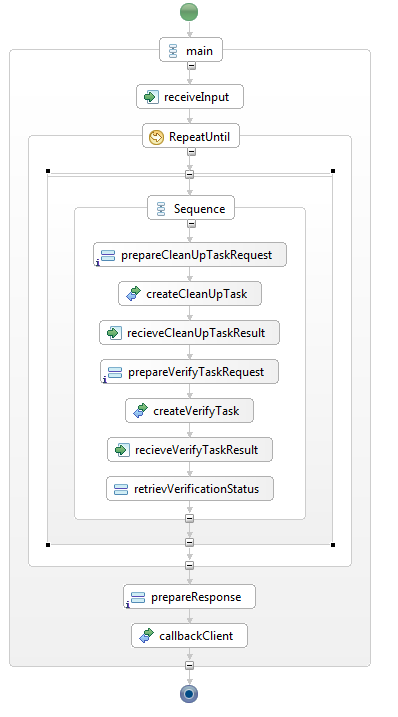
\includegraphics[scale=0.6]{bpelProcess}}
\caption{Wizualizacja procesu BPEL w postaci graficznej za pomocą wtyczki do Eclipsa.}
\label{fig:bpelProcess}
\end{figure}

Do implementacji procesu BPEL została wykorzystana wtyczka do zintegrowanego środowiska programistycznego Eclipse. Wtyczka ta udostępnia narzędzia do modelowania procesów BPEL w sposób graficzny. Na rysunku~\ref{fig:bpelProcess} został przedstawiony zrzut ekranu przedstawiający implementację niniejszego procesu biznesowego. Na rysunku widać doskonale kolejność wywoływania poszczególnych aktywności procesu BPEL, nie widać natomiast zastosowania mechanizmu korelacji oraz zakresu. 

\subsubsection{Korelacja}

Mechanizmem na który w szczególności należy zwrócić uwagę podczas opisu procesu biznesowego jest mechanizm korelacji. Mechanizm ten służy do powiązania dwóch lub więcej operacji wewnątrz jednej instancji procesu. W przypadku niniejszego przykładu proces korelacji wykorzystywany jest do powiązywania operacji stworzenie zadania z operacją odebrania rezultatu zadania. Zazwyczaj środowisko uruchomieniowe posiada więcej niż jedną instancje procesu, w momencie gdy zostaje odebrany rezultat zadania np. sprzątania środowisko powinno w jakiś sposób zidentyfikować instancję procesu do której zaadresowany jest ten rezultat. 

Mechanizm korelacji realizowany jest za pomocą tak zwanych zbiorów korelacji. Zbiór korelacji nie jest niczym innym jak zbiorem zmiennych. Zmienne te inicjalizowane są przy pierwszym użyciu dowolną wartością, podczas kolejnego użycia służą do odszukania instancji procesu o zadanej wartości. 

W niniejszym procesie istnieją dwa zbiory korelacji, zdefiniowane wewnątrz ciała pętli: 

\begin{lstlisting}[caption=Definicja zbiorów korelacji.,numbers=left]
<bpel:correlationSets>
	<bpel:correlationSet name="cleanUpTask" 
			properties="tns:taskUUID"/>
	<bpel:correlationSet name="verifyTask" 
			properties="tns:verifyTaskUUID"/>
</bpel:correlationSets> 


\end{lstlisting}

Zbiory te wykorzystywane są do powiązania operacji stworzenia i odbioru rezultatu zadania sprzątanie i weryfikacja. 

\begin{lstlisting}[caption=Wykorzystanie zbiorów korelacji w aktywności invoke.,numbers=left]
<bpel:receive name="recieveCleanUpTaskResult" partnerLink="client" 
	operation="cleanUpTaskCallback" portType="tns:cleanUpProcess" 
	variable="clientRequest">
            <bpel:correlations>
                <bpel:correlation set="cleanUpTask" initiate="no">
	     </bpel:correlation>    
            </bpel:correlations>
        
</bpel:receive>
\end{lstlisting}

Operacja invoke odpowiedzialna za stworzenie zadania inicjalizuje zbiór korelacji odebraną z warstwy pośredniej wartością unikalnego identyfikatora zadania.

\begin{lstlisting}[caption=Wykorzystanie zbiorów korelacji w aktywności receive.,numbers=left]
<bpel:receive name="recieveCleanUpTaskResult" partnerLink="client" 
		operation="cleanUpTaskCallback"
	          portType="tns:cleanUpProcess" variable="clientRequest">
            <bpel:correlations>
                	<bpel:correlation set="cleanUpTask" initiate="no">
		</bpel:correlation>    
            </bpel:correlations>
</bpel:receive>

\end{lstlisting}

 Operacja recieve następnie na podstawie tego samego unikalnego identyfikatora odnajduje odpowiednią instancje by kontynuować jej działanie. 

\subsubsection{Zakres }
Bezpośrednio powiązany z mechanizmem korelacji jest mechanizm zakresów. Służy on do odizolowania dwóch lub więcej operacji wewnątrz procesu. Izolacja ta może zostać wykorzystana np. do odpowiedniego zarządzania sytuacjami wyjątkowymi. W przypadku niniejszego procesu mechanizm zakresu został zastosowany do odizolowania kolejnych wywołań pętli w celu uzyskania efektu ponownej inicjalizacji zbiorów korelacji w każdym przebiegu pętli. W przypadku nie zastosowania mechanizmy zakresu, podczas pierwszego wywołania przebiegu pętli zbiór korelacji zostałby zainicjalizowany identyfikatorem pierwszego zadania. W przypadku kolejnych wywołań pętli metoda reciev oczekiwała by na identyfikator pierwszego zadania mimo, że zostało ono już rozwiązane a kolejny przebieg pętli stworzył następne zadanie. 

Mechanizm zakresu stosuje się obejmując izolowane elementy w drzewie xml elementem: 

\begin{lstlisting}[caption=Przykład zastosowania zakresu w BPEL.,numbers=left]
<bpel:scope isolated="yes">
...
</bpel:scope>
\end{lstlisting}

\subsection{Uruchomienie}
 Proces BPEL został stworzony zgodnie ze specyfikacją BPEL, może być zatem wdrożony na dowolne środowisko uruchomieniowe dla procesów biznesowych. W przykładzie zastosowano środowisko Apache ODE. 

Apache ODE jest również aplikacją internetową napisaną w języku Java i może być uruchomiony z wykorzystaniem dowolnego serwera aplikacyjnego. Ważne jest aby silnik Apache ODE został uruchomiony z wykorzystaniem portu 8080. System Zarządzania Hotelem będzie próbował uruchomić proces na lokalnej maszynie pod tym właśnie portem.  


%---------------------------------------------------------------------------

\section{Warstwa pośrednia }
\label{sec:exampleMiddleware}


%---------------------------------------------------------------------------

\section{Aplikacja mobilna}
\label{sec:exampleMobileApp}

Aplikacja mobilna jest częścią przykładu odpowiedzialną za rozwiązywanie zadań poprzez udostępnienie użytkownikom odpowiedniego interfejsu. Aplikacja komunikuje się w warstwą pośrednią za pomocą REST API w celu pobrania listy zadań, operacji na tych zadaniach i wysłania rezultatu. Aplikacja została zaimplementowana na najbardziej popularną platformę mobilną - Android. 

Aplikacja wykorzystuje specyficzny dla tej platformy mechanizm synchronizacji zarządzany przez system operacyjny. Synchronizacja uruchamiana jest bez konieczności działania aplikacji w momencie gdy urządzenie ma dostęp do sieci. Przez synchronizacje w tym wypadku rozumiane jest pobranie listy zadań dostępnych dla użytkownika i ich zapis w lokalnej bazie danych (SQLite). Aplikacja przewiduje możliwość logowania więcej jak jednego użytkownika, dane każdego z nich zapisywane są do osobnej bazy danych. Użytkownik po wejściu do aplikacji widzi listę dostępnych dla niego zadań mimo, że może nie mieć dostępu do sieci. Użytkownik może zadeklarować chęć wykonania zadania oraz w momencie gdy jest do niego przypisany rozwiązać je klikając odpowiednie przyciski.

\subsection{Wybrane technologie}

Aplikacja została zrealizowana z wykorzystaniem język Java, platformy Android, bibliotek Spring  for Android oraz OrmLite. 

\subsection{Implementacja}


\begin{thebibliography}{1}

%\bibitem{Dil00}
%A.~Diller.
%\newblock {\em LaTeX wiersz po wierszu}.
%\newblock Wydawnictwo Helion, Gliwice, 2000.
%
%\bibitem{Lam92}
%L.~Lamport.
%\newblock {\em LaTeX system przygotowywania dokumentów}.
%\newblock Wydawnictwo Ariel, Krakow, 1992.
%

\bibitem{EAOBPMWeb}
European Association of Business Process Management.
\newblock {\em {Organization home website}}.
\newblock \\\texttt{http://www.eabpm.org/}.


\bibitem{wiBPMA}
Antipodes.
\newblock {\em {What is a Business Process Management system?}}.
\newblock \\\texttt{http://www.antipodes.bg/en/cubes/what\_is\_bpm/}.

\bibitem{OASISweb}
OASIS.
\newblock {\em {OASIS Web Services Business Process Execution Language (WSBPEL) TC}}
\newblock \\\texttt{https://www.oasis-open.org/committees/tc\_home.php?wg\_abbrev=wsbpel}

\bibitem{OASISBPELSpec}
OASIS
\newblock {\em Web Services Business Process Execution Language Version 2.0}.
\newblock OASIS Standard 11 April 2007 

\bibitem{wiao}
Mulesoft.
\newblock {\em {What is application orchestration?}}
\newblock \\\texttt{http://www.mulesoft.org/what-application-orchestration}

\bibitem{bpel4People}
IBM and SAP.
\newblock {\em WS-BPEL Extension for People – BPEL4People}.
\newblock A Joint White Paper by IBM and SAP July 2005 

\bibitem{rest}
Patryk Yarpo Jar
\newblock {\em {REST – ciekawszy sposób na komunikację client-server}}
\newblock \\\texttt{http://www.yarpo.pl/2012/07/29/rest-ciekawszy-sposob-na-komunikacje-client-server/}

\end{thebibliography}

\end{document}
